\chapter{Introduction}

\section{The Case for New Solar Absorber Materials for Photovoltaic Devices}

\subsection{Terawatt-Scale Power Production from Renewable Resources}

It is now widely accepted that the world is heading towards a major energy crisis, where there will come a point that the current major sources of energy (namely fossil fuels) will be unable to meet increasing global demand for energy as they are not a limitless supply. Furthermore, there is the ever present worry of climate change linked to increased carbon dioxide emissions from the burning of fossil fuels. Renewable, low-carbon alternative energy sources are therefore clearly desirable. From purely environmental considerations, it seems clear that fossil fuels should no longer be used and we should meet our energy needs solely from renewable, low-carbon energy resources such as solar power. However, it is not only environmental sustainability that must be considered, we must also consider the economic feasibility of solar power for large-scale projects. Germany is an example of a country making considerable efforts to increase the percentage of their energy supplied by solar power. On 9 June 2014 Germany even generated over 50\% of its electricity demand from solar for the first time \cite{Germany_guardian_news}. Although on average the country is not able to produce such a large portion from solar power, with solar-generated power providing approximately 7.5\% of net electricity consumption in 2015 \cite{Germany_PV}. To facilitate the growth of the solar power capacity in Germany a number of schemes and financial incentives to encourage investment were introduced, such as feed-in tariffs (FiTs).
The German government first introduced FiTs in their Grid Feed-In Law (the Stromeinspeisegesetz), which came into force in 1991 \cite{Germany_Lang}. FiTs are intended to support new developments in renewable energy supply by providing investor certainty. They set the rate a utility company must pay for renewable generated energy and guarantee the provider of renewable energy a specific rate for a long period of time, typically fifteen to twenty years. As this cost is higher than fossil fuel based electricity, the higher price is then passed on to all customers of the utility company to spread out the higher costs so that buyers of renewable energy do not pay higher prices. In Germany, this has resulted in an increase of 6\% on the average electricity bill for users in a specific region \cite{Germany_Oregon}. The social implications of such a cost increase must also be considered in assessing the viability of a particular power source.\\

\begin{figure}[h!]
  \centering
    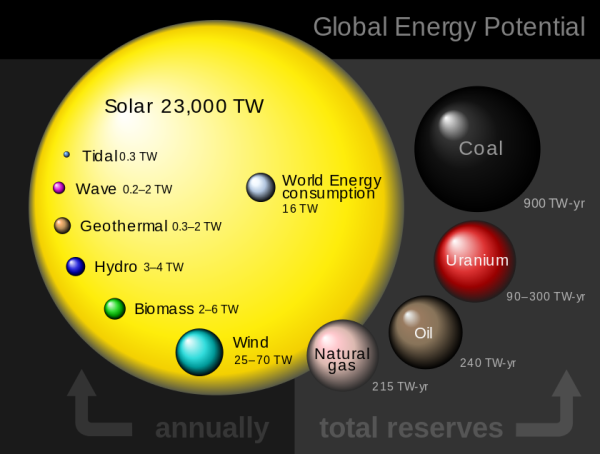
\includegraphics[width=0.75\textwidth]{figures/global_energy.png}
    \caption{Illustration of power available annually from various renewable energy resources, annual world energy consumption and total reserves of various non-renewable energy resources. Figure take from reference \citenum{global_energy_fig}.}
  \label{global_energy}
\end{figure}

However if solar power, in combination with proper energy transport, storage and secondary conversion into heat and fuels, could be made to be economically feasible; it is a realistic candidate for replacing fossil fuels as a major supply of global energy. It is by far the largest source of energy available to us, as illustrated in figure \ref{global_energy}, and it is also the most widely geographically distributed \cite{inorg_pv}. The Sun supplies $3 \times 10^{24}$ J of energy to the Earth each year, which is around $10^4$ times more than mankind's current annual energy consumption. 
Assuming a fairly modest module efficiency of 20\%, a system capacity factor of 15\%, an average ground cover ratio of 50\%, and 50\% losses related to storage and secondary conversion, 1.6\% of the Earth’s land area would be required for solar-generated power to meet current world energy needs \cite{newPVrev}. Although this would be a fairly large area, it would not be completely unrealistic. For instance, this area would be less than 5\% of the area used for agriculture worldwide \cite{newPVrev}. The area required could also be reduced further through improvements in the efficiency of PV module and by making use of building-integrated PV (BIPV) innovations, largely made possible by flexible, thin-film second generation PV technologies which are discussed further in section \ref{current_tech}. An example of a BIPV project is shown in figure \ref{BIPV}, where solar panels are not only placed on the roof of a building but can also placed on the windows and outer walls.\\ 

\begin{figure}[h!]
  \centering
    \includegraphics[width=0.75\textwidth]{figures/BIPV.jpg}
    \caption{A building integrated photovoltaics (BIPV) project fitted in the United States by BISEM-USA \cite{BIPV}.}
  \label{BIPV}
\end{figure}

Recent years have seen a rapid increase in the installed solar generation capacity, with the global grid-connected PV capacity growing from 1.3 GW in 2000 to 139 GW in 2014 \cite{pathways_129}, with approximately a doubling in the cumulative installed capacity every two years \cite{pathways}. Additionally, creative business models have spurred investment in residential solar systems \cite{MIT}. Great improvements in technology, price and performance have helped to facilitate this growth, but solar energy still only provides a minor fraction of the world's energy. In 2013 solar power only provided 0.87\% of the worlds electricity \cite{pathways_130}. Further advances are required to enable a dramatic increase in the contribution from solar power at socially acceptable costs \cite{MIT}. Ultimately, solar power-generation technologies must become cost-competitive with conventional fossil-fuel based power sources.\\

\begin{figure}[h!]
  \centering
    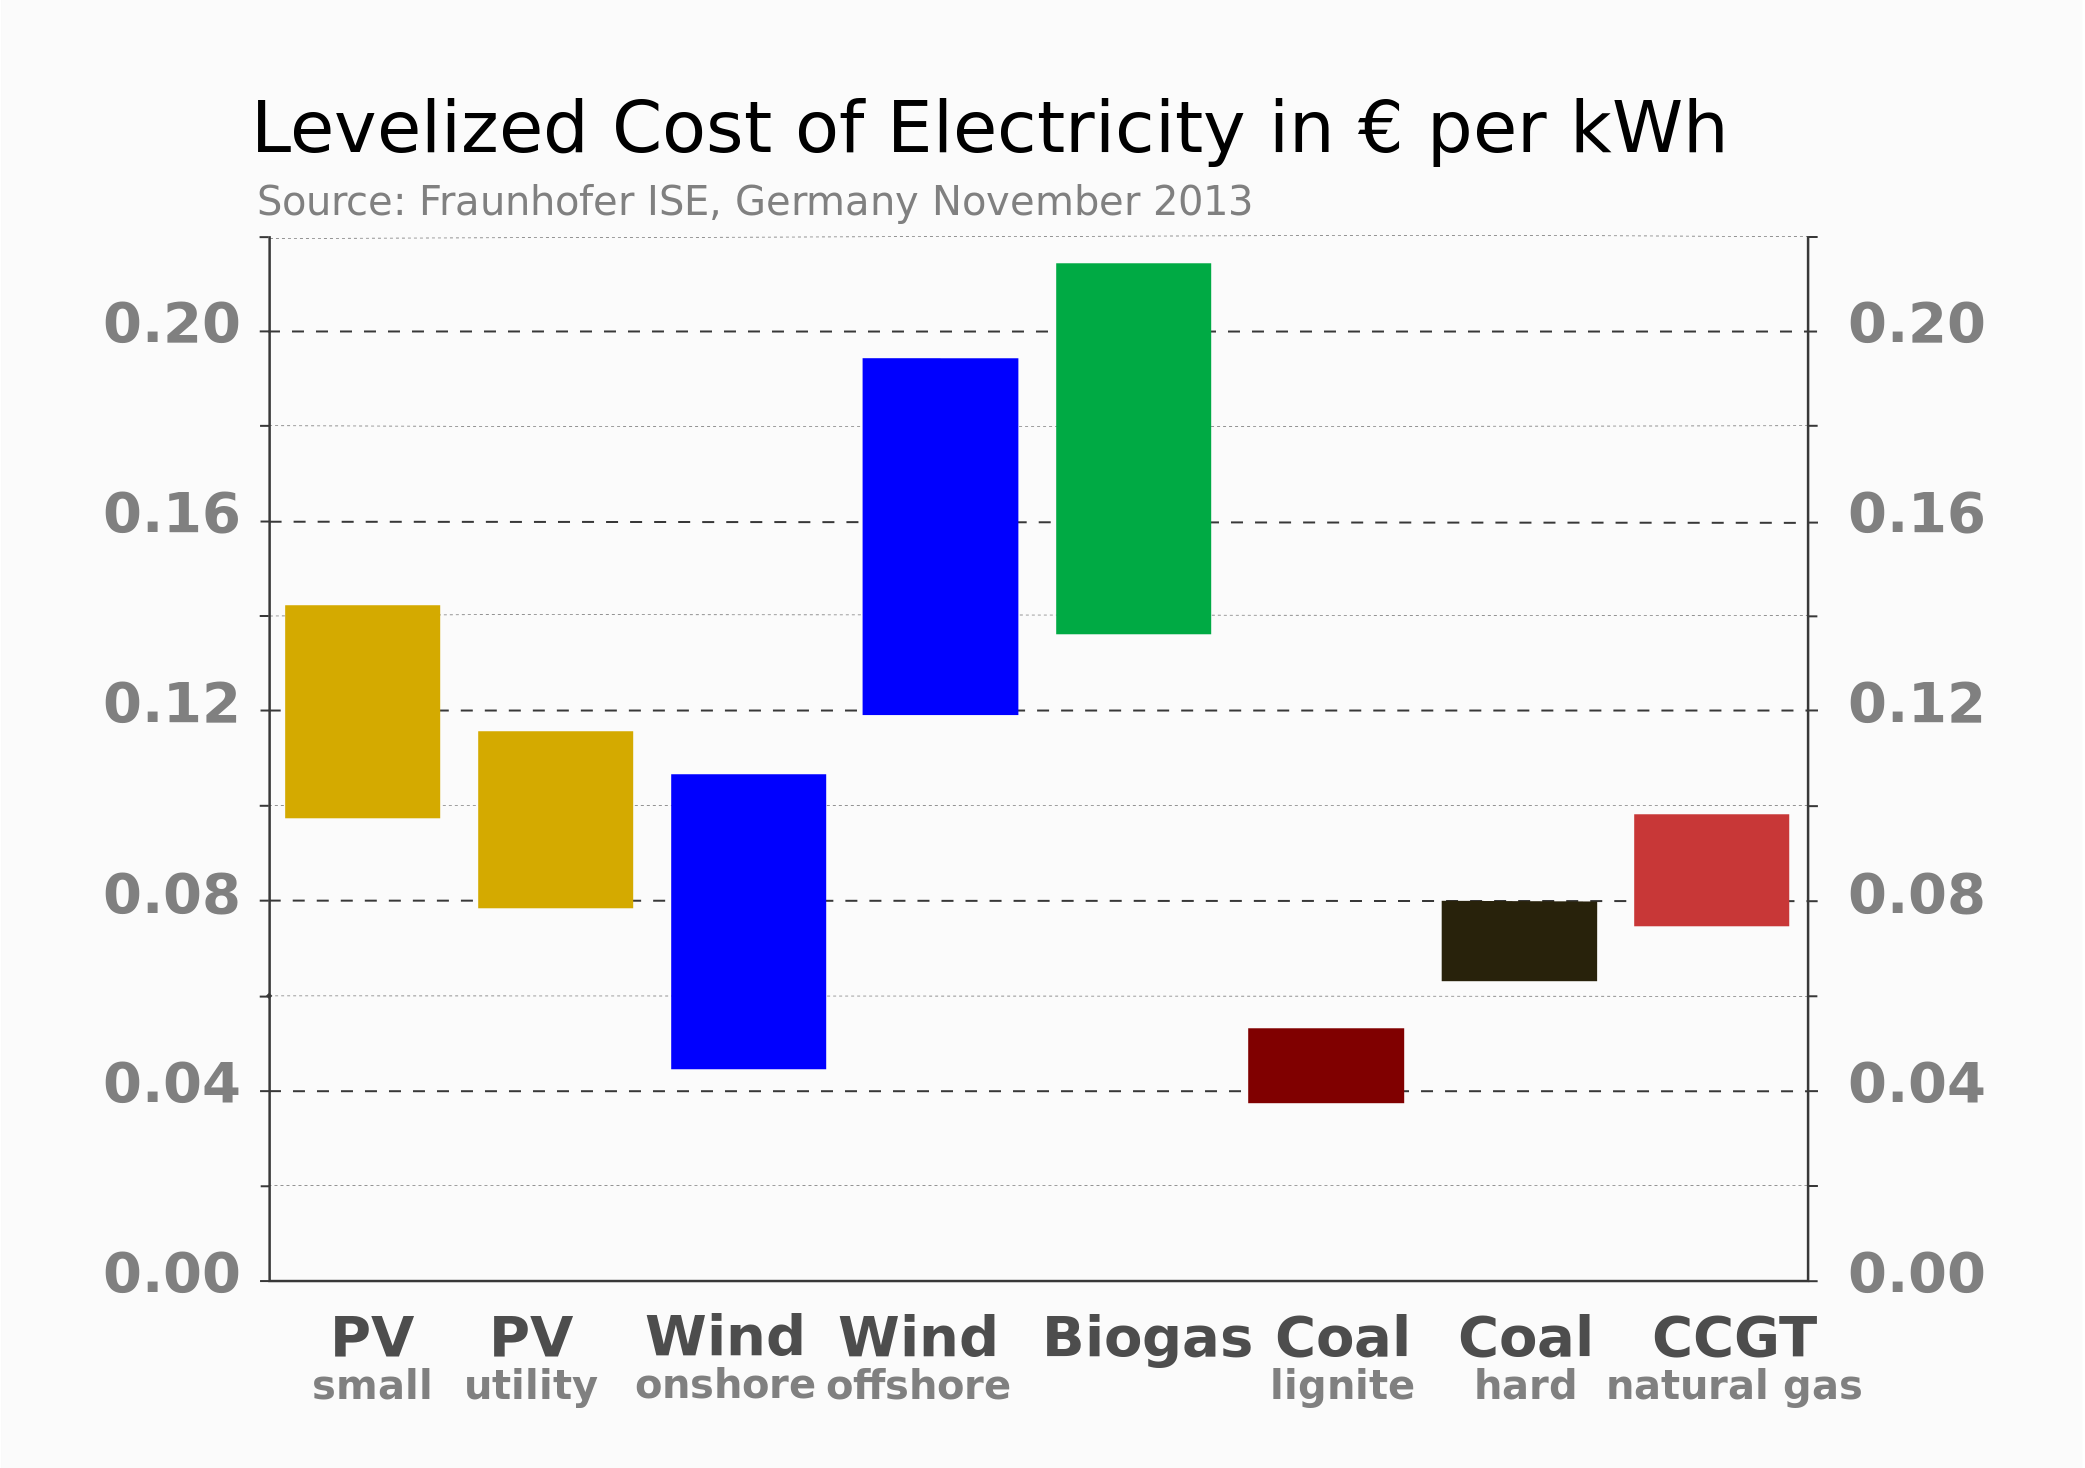
\includegraphics[width=0.8\textwidth]{figures/LCOE.png}
    \caption{Levelized cost of electricity (LCOE) of renewable energy technologies and conventional power plants at locations in Germany in 2013.  Specific investments are taken into account with a minimum and maximum value for each technology. Figure taken from reference \citenum{LCOE}.}
  \label{LCOE}
\end{figure}

Levelized cost of energy, or electricity, (LCOE) is a common way to assess how cost competitive renewable energy sources are with their non-renewable counterparts. LCOE allows for the measurement of the performance of different power generating technologies, which may have unequal lifetimes and differing capacities. It is calculated by summing all costs incurred during the lifetime of the technology and dividing this value by the units of energy produced during the lifetime, with units of energy expressed as dollars per kilowatt hour (\$/kWhr) \cite{LCOE2}. This measure is also used as the key selling point for a number of commercial solar cell manufacturers such as First Solar Inc., who market their product as being able to generate electricity at an average of \$0.63 per Watt as stated in their 2013  Annual Report \cite{first_solar}. Using the LCOE, comparisons of grid competitiveness for renewable energy sources can be made \cite{LCOE2}. Figure \ref{LCOE} shows the LCOE of renewable energy technologies and conventional power plants at locations in Germany in 2013, enabling an assessment of the cost-competitiveness of PV power generation at this location, accounting for, for example, typical solar irradiation at the given locations \cite{LCOE}. As the figure shows, both small-scale and large-scale utility solar power are still not cost competitive with the cheapest non-renewable resources.\\




\subsection{Basic Operating Principles of a Solar Cell Device}\label{basic_PV}
Refer to: pg 5 \cite{spatial_resolved_book}, pg 11 + 18 \cite{PV_Goetzberger}\\


\begin{figure}[h!]
  \centering
    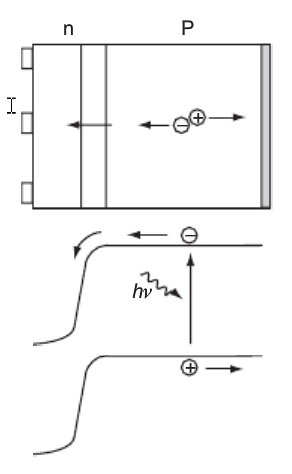
\includegraphics[width=0.45\textwidth]{figures/PV_schematic.png}
    \caption{Schematic of a typical crystalline silicon solar cell device (top), where the majority of the cell consists of a thick p-type base in which most of the light is absorbed.  After light absorption, the minority carriers (electrons) diffuse to the junction where they are swept across by the strong built-in electric field. The electrical power is collected by metal contacts to the front and back of the cell. Excitation of an electron-hole pair across the band gap of the p-type material (bottom). 
    Figure taken from reference \citenum{PV_handbook}.}
  \label{PV_schematic}
\end{figure}

A solar cell device converts solar energy directly into electrical energy, where solar energy can be described as either a spectrum of electromagnetic radiation or a flux of photons ???(and electrical energy is a flow of charge carriers able to do work in an external circuit.)??? \cite{spatial_resolved_book} Voltage is generated in a solar cell device by the photovoltaic effect. The terms `solar cell' and `photovoltaic (PV) cell' are therefore often used interchangeably.  

Semiconducting materials are usually utilized in a PV device. A semiconductor is described by its valence and conduction energy
bands i.e. a group of energy levels, which electrons may occupy, and a gap in
between with no available energy levels called the bandgap. In thermal equilibrium
at a 0 K, all the energy levels in the valence band are occupied by electrons
while all energy levels in the conduction band remain unoccupied. Energy level
occupancy at temperais usually described by the Fermi-Dirac distribution [1]. \cite{spatial_resolved_book}

Only photons with energies higher than the bandgap can be absorbed in the
perfectly pure semiconductor by exciting an electron from the valence to the conduction
band, while simultaneously conserving total energy and momentum. Two
types of semiconductors are distinguished with regards to the shape of the valence
and conduction band in the energy–momentum diagram. In a direct semiconductor,
the maximum energy of the valence band and the minimum energy of the conductance
band are located at the same momentum, which is not the case in an indirect
semiconductor. Light absorption in a direct semiconductor occurs when the
photon interacts with only an electron from the valence band. Light absorption
in an indirect semiconductor requires a phonon (i.e. a quantum of thermal energy
with considerable momentum, which is discernible as a crystal lattice vibration)
assisted transition, where a phonon provides or consumes the difference in momentum. \cite{spatial_resolved_book}


When semiconducting materials absorb photons of light with energies of at least their band gap, electrons are excited to higher energy states within the material to 
form an electron-hole pair, as shown in figure \ref{PV_schematic}. The excited electron-hole pair would eventually recombine and relax back 
to the ground state of the material with the emission of a photon of an energy equal to the energy of the 
electronic transition that has just occurred. 
However in a PV device, there is a built-in asymmetry that leads excited charge-carriers away before they can recombine back to the ground state. The extra energy of the excited electron generates a potential difference that drives electrons through a load in the external circuit to 
do electrical work. In the conventional PV effect, as electrons are excited across the band gap of a semiconductor, the band gap of the material sets the upper limit for the maximum voltage that can be generated. In early PV devices, the asymmetric junction was a Schottky barrier between a metal and a 
semiconductor but now more effective p-n junctions are used, which are formed by joining together p-type and n-type semiconductors \cite{Nelson1}. \\

\begin{figure}[h!]
  \centering
    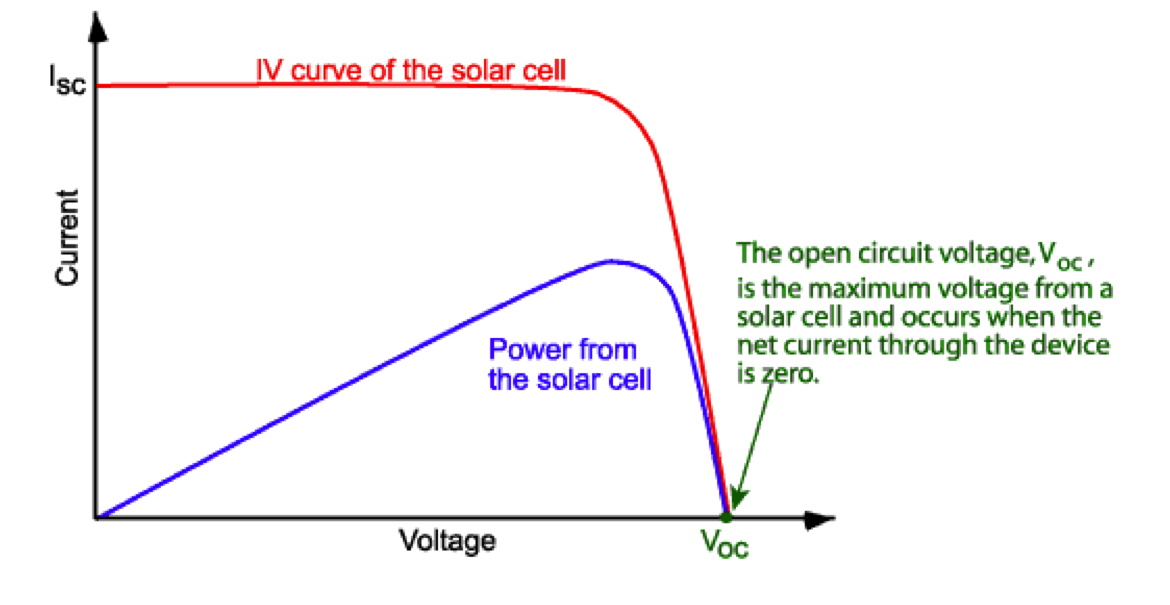
\includegraphics[width=0.65\textwidth]{figures/IV}
    \caption{The current-voltage (I-V) curve of a solar cell showing the open circuit voltage ($V_{OC}$). Figure taken from reference \citenum{PVeducation}.}
  \label{IV}
\end{figure}

When a cell consisting of a p-n junction is illuminated, a voltage develops across the terminals, i.e. between the p-type and n-type semiconductors. When the terminals of the solar cell are disconnected from any external circuit, or there is an infinite load resistance, this voltage is at a maximum and is called the open circuit voltage ($V_{OC}$) and no current is drawn from the solar cell. Conversely, if the terminals of the solar cell are connected together then there is no voltage as all of the electromotive force is used to extract charge-carriers. The maximum possible current is drawn, which is called the short circuit current ($I_{SC}$). For a solar cell to generate power, there must be both voltage and current generated, therefore when the cell is operating at either $V_{OC}$ or $I_{SC}$ the power output is zero. To generate power, a finite load resistance is added to the circuit so that some current is drawn from the solar cell and a voltage develops across the cell that is between 0 and $V_{OC}$ \cite{Nelson1}. There is a maximum operation point for the power output ($P_{MP}$) of a solar cell in terms of I and V, as shown in figure \ref{IV}. This can be defined in terms of $V_{OC}$ and $I_{SC}$ when used in conjunction with the fill factor (FF), which is a number less than one that describes the squareness of the I-V curve \cite{handbook} shown in figure \ref{IV} and is given by equation \ref{P_MP}. The current and voltage are determined by the load and illumination so the load can be tuned such that maximum power output is achieved, but the value of $V_{OC}$ places a limit on the power output of the cell \cite{Nelson1}.

\begin{equation} \label{P_MP}
P_{MP} = FFV_{OC}I_{SC}
\end{equation}

\begin{equation} \label{efficiency}
\eta = \frac{P_{MP}}{P_{in}} = \frac{FFV_{OC}I_{SC}}{P_{in}}
\end{equation}

The power conversion efficiency (PCE), $\eta$, of a solar cell is the ratio of power output from the solar cell to the power input from the Sun. This is shown in equation \ref{efficiency}, where $P_{MP}$ has been taken from equation \ref{P_MP}.
For an efficient solar cell, it is desirable to have a high $I_{SC}$, a high $V_{OC}$ and a FF that is as close to 1 as possible \cite{handbook}. \\

**Move discussion to section on candidate new materials** CZTS solar cells are known to be hampered by low $V_{OC}$ relative to the band gap of the material \cite{SS}. Whereas in ferroelectric PV materials, photovoltages orders of magnitude larger than the band gap have been measured (a phenomena referred to as the anomalous photovoltaic effect), but very low photocurrent output is a big challenge for these devices \cite{FE_PV_rev1}.\\

**Add figure and description of basic PV device + show basic simplified band diagram (later compare to real band structure, e.g. of Si**\\

A solar cell device consists of... (see Mirjana's thesis)

** Explicitly discuss recombination

\subsection{Key Properties for Solar Absorber Materials}\label{PV_properties}

A solar (or photovoltaic) cell is an example of an optoelectronic device in which the solar absorber material of choice must allow for the manipulation of light, electrical current and their interaction. Metals are excellent electrical conductors, but do not allow light to travel inside. Glass and related dielectric materials can accommodate and guide light waves, as in electrical fibres, but are electrical insulators. Semiconductors are in between these two types of material as they can carry both electrical current as well as light waves \cite{mat_prop1}. Furthermore, some semiconductors can be used to transform light into electrical current, which was described in the section above. The two vital processes that must occur in a solar absorber material were also discussed above, which were: the excitation of an electron across the band gap from the valence band into the conduction band in a semiconducting material by a photon and the subsequent collection of the photoexcited charge carriers by an external circuit before the photoexcited electron-hole pair recombine. There are certain optical and electrical properties that are necessary for these processes to occur and then there are also certain properties that indicate how well a material is likely to perform in a solar cell device. In this section the band gap, effective mass, dielectric constant and absorption coefficient of a potential solar absorber material will be discussed.

\begin{figure}[h!]
  \centering
    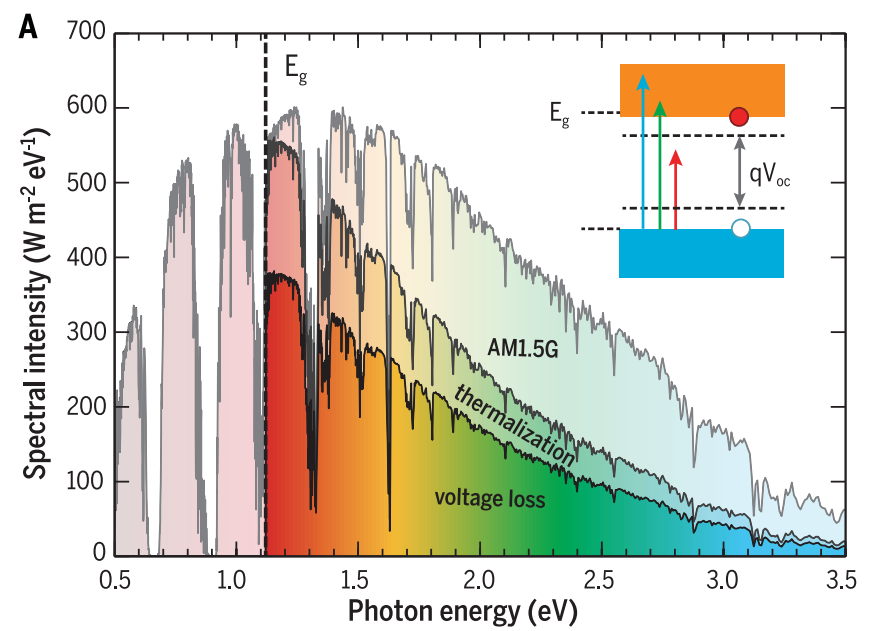
\includegraphics[width=0.85\textwidth]{figures/solar_spectrum2.png}
    \caption{AM1.5 solar spectrum with distinct dips due to molecular absorption in Earth’s atmosphere. The dashed line shows the band gap of silicon and fading to the left indicates that photons with energies below the band gap will not be absorbed and other fading indicates other loss mechanisms that prevent a solar cell from being unable to convert the full incident spectrum into electricity. Figure taken from reference \citenum{newPVrev}.}
  \label{solar_spectrum}
\end{figure}

\begin{figure}[h!]
  \centering
    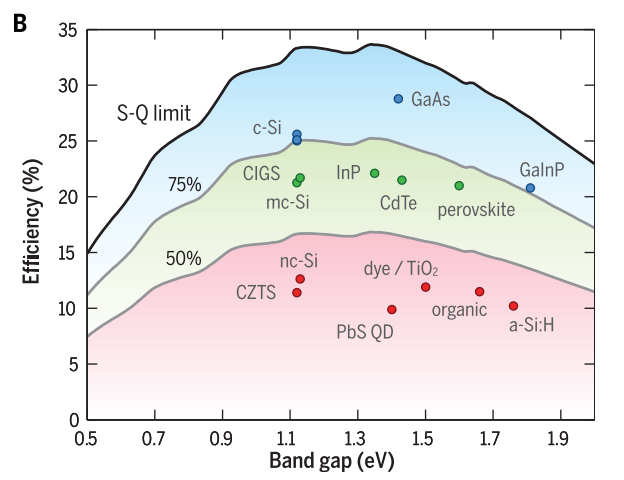
\includegraphics[width=0.65\textwidth]{figures/SQ_new.png}
    \caption{Theoretical Shockley-Queisser detailed-balance efficiency limit as a function of band gap\cite{SQ_1961} (highest black line). The record efficiencies for different materials are plotted for the corresponding band gaps, where materials below the lower two grey lines are achieving conversion efficiencies less than 75\% and 50\% of their theoretical efficiency limit respectively. Figure taken from reference \citenum{newPVrev}.}
  \label{SQ}
\end{figure}

The most obvious necessary requirement for a solar absorber material is for it to be a semiconductor so that it possesses a band gap across which an electron can be excited. The value of this band gap must also be somewhere within the energy range of the solar spectrum shown in figure \ref{solar_spectrum}, so that sunlight can induce the photoexcitation of an electron-hole pair across the band gap. Secondly the material must allow for the transport of charge carriers out of the absorber material and into a collection electrode and external circuit in order to do electrical work. Provided these necessary conditions are met and some sort of bias is applied to drive the separation of the electron-hole pair, the material should exhibit the photovoltaic effect. However, how well it will actually peform in a solar cell is determined by more stringent criteria and other material properties. Firstly the actual value of the band gap within the range of the solar spectrum is of importance. It is ideal for the value to be as close as possible to the region of photon energies that make up the majority of the solar spectrum. The optimal range for the band gap under typical radiation conditions is between 1.06 eV and 1.50 eV \cite{CZTS_book}. The upper limit of the power conversion efficiency (of incident photon energy into electrical energy) by a device made from a particular absorber material based on its band gap was first calculated by Shockley and Quiesser in 1961 \cite{SQ_1961}. A plot of theoretical efficiency limit as a function of band gap is shown in figure \ref{SQ}.

However, it is not only the value of the band gap that is of importance. More intricate details of the band structure of the material can also impact on the performance of a solar cell device made from the material. Band theory and band structures will be discussed more in section \ref{band_theory}, but it is worth noting at this point that if the band structure shows a band gap that is direct or indirect can have an impact on the performance of a solar cell made from the material. Figure \ref{Si_and_GaAs} shows the band structures of Si and GaAs, where Si possesses an indirect band gap and GaAs possesses a direct band gap. The excitation of an electron directly from the valence band to the conduction band is called fundamental absorption, as there are several other optical absorption transitions that can occur in a semiconducting material, especially in a defective material, and this point will be discussed more in section \ref{PL_section}. Both the total energy and moment of all particles involved in the absorption process must be conserved. Photons do possess momentum ($\frac{h}{\lambda}$), however this is very small compared to the range of crystal momenta and so the electron momentum is effectively conserved during photon absorption. For a direct transition, the absorption coefficient of a material for a given photon energy $h \nu$ is proportional to the probability, p$_{12}$, of the transition of an electron from the initial state E$_1$ to the final state E$_2$, the density of electrons in the initial state, $g_{v}(E_1)$, and the density of available final states, $g_{c}(E_2)$. This is then summed over all possible transitions between states where $E_2 - E_1 = h\nu$. Since the electron momentum is conserved during a direct transition, the crystal momentum in the valence band is approximately the same as that of the final state in the conduction band at energy $E_2$ \cite{PV_bands_book}.

However for an indirect band gap semiconductor, such as silicon shown at the top of figure \ref{Si_and_GaAs}, the valence band maximum occurs at a different crystal momentum to that of the conduction band minimum. As discussed earlier, the momentum of a photon is far less than that of crystal momenta. In order to conserve the momentum of an electron during an optical transition across an indirect band gap, momentum must be either provided by the lattice or released to the lattice in the form of the particle representation of a lattice vibration, known as a phonon, as indicated in the top right schematic of figure \ref{Si_and_GaAs}. Since both a phonon and an electron are needed to make an indirect transition possible, the absorption coefficient depends not only on the density of states of the electrons, as for a direct transition, but also on the availability of emitted or absorbed phonons with the required momentum. Therefore, the absorption coefficient for an indirect transition compared to a direct transition is typically relatively small. Consequently, light penetrates more deeply into an indirect band gap semiconductor before being absorbed. In order to absorb the same amount of light therefore, the absorber layer of a device made from an indirect band gap semiconductor must therefore typically be thicker \cite{PV_bands_book}. This is undesirable if the particular material contains rare or expensive components and also results in higher demands on material quality as charge carriers must be able to be transported through the absorber material in order to be collected.

\begin{figure}[h!]
  \centering
    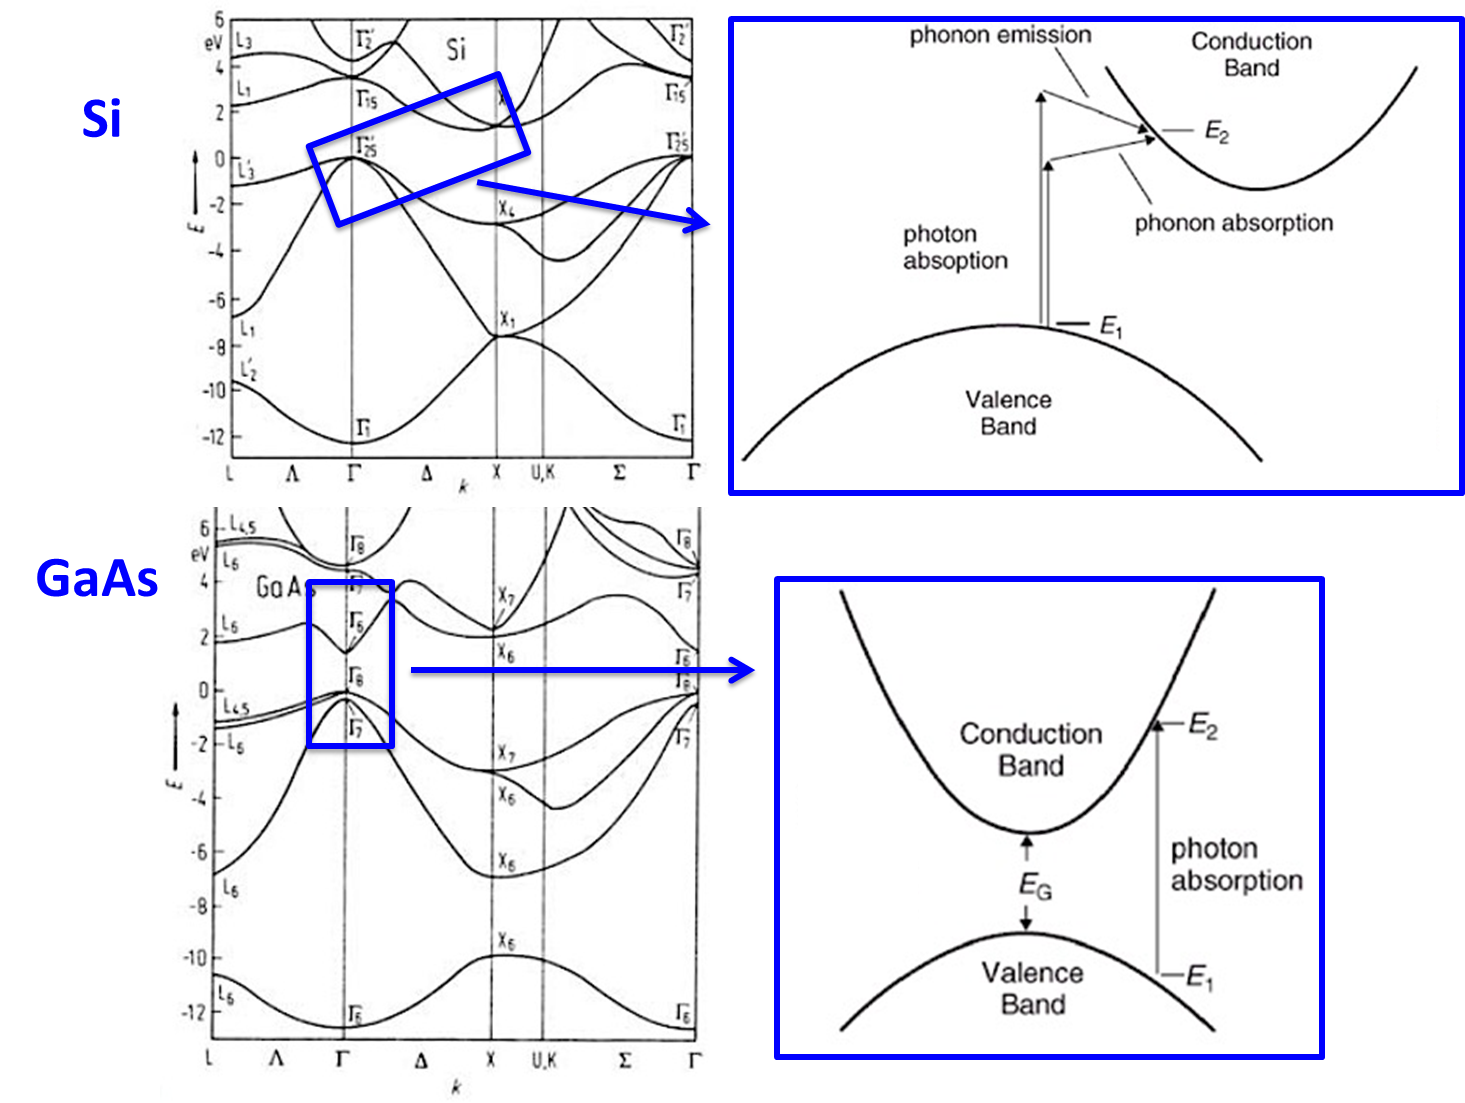
\includegraphics[width=0.95\textwidth]{figures/Si_and_GaAs.png}
    \caption{The band structure of silicon and a schematic of the absorption process in an indirect band gap semiconductor (top). The band structure of GaAs and schematic of the absorption process in a direct gap semiconductor. Figures adapted from \citenum{phys_semicond} and \citenum{PV_bands_book}.}
  \label{Si_and_GaAs}
\end{figure}

Another property of importance that can be derived from the band structure of a material is the effective mass. The effective mass is related to the curvature of the band at the top of the valence band (for holes) or at the bottom of the conduction band (for electrons). The effective masses of electrons or holes are the masses they seem to carry for transport properties \cite{dielectric_const1}. For example, in ZnSnO$_3$ the hole effective mass has been calculated to be large, indicating that hole mobility will be poor in this material. Poor mobility will make carrier extraction difficult, which has been linked to the low photocurrents observed in this material \cite{effective_mass1}. Effective masses are calculated by fitting a formula, which will be discussed more in the methodology section \ref{properties_methods}. However, just from a quick inspection of the band structure of a material, a more steeply curved shape to the band extrema indicates a lower effective mass and therefore higher carrier mobility. Figure \ref{heavy_holes} shows a schematic of the band structure of a direct band gap semiconductor that has both heavy- and light-hole bands at the valence band extremum, where the flatter band correponds to the heavy-hole band.
Although certain thin-film technologies, which will be discussed towards the end of section \ref{current_tech}, reduce the amount of absorber material the charge carrier must travel through before being collected. So although carriers must still travel through the material, effective mass could be considered less of a crucial parameter for this technology. Furthermore, the effect of the effective mass on the transport properties could be overshadowed by the effect of defects in a real, non-ideal material. It is the dielectric function of the material that provides more insight in this case, which is discussed below.

\begin{figure}[h!]
  \centering
    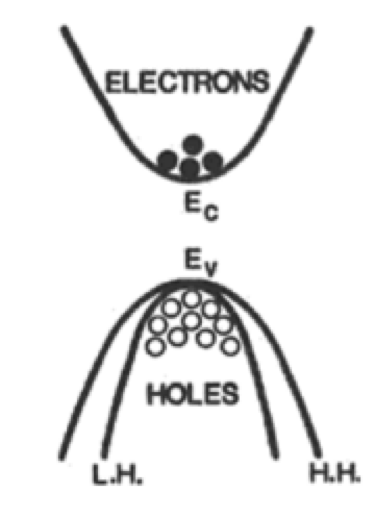
\includegraphics[width=0.3\textwidth]{figures/heavy_holes.png}
    \caption{Schematic of a the band structure of a photoexcited semiconductor with electrons near the bottom of the conduction band, holes near the top of the valence band, where the particular material has both heavy- and light-hole bands (labelled H.H and L.H in the figure respectively). Figure taken from reference \citenum{heavy_holes}.}
  \label{heavy_holes}
\end{figure}

Materials with ionic or covalent bonding, or a mixture of the two, are usually either insulators or intrinsic semiconductors. Due to this type of bonding, electrons are bound to the atomic structure and so are unable to move throughout the material when an electric field is applied as in a metal. However, these materials can be polarized by an applied electric field where electrons are displaced relative to their nuclei by small distances. When an external electric field is applied, the positive and negative charges experience electric forces tending to move them apart in the direction of the external field so that their centres of gravity no longer coincide \cite{dielectric2}. The material is now said to be polarized and an electric displacement field ($\vec{D}$) appears within it. The applied field ($\vec{E}$) and displacement field are linked by the macroscopic dielectric function of the material, $\epsilon_r$, as shown by equation \ref{displacement_field} \cite{dielectric_const1}, which is a function of the frequency of the applied field.
\begin{equation} \label{displacement_field}
\vec{D} = \epsilon_0 \epsilon_r \vec{E}
\end{equation}
The dielectric function indicates the ability of a material to screen the external electric field by the apparition of a polarization. In a solid, this polarization comes from the re-organization of the electronic density or from the motion the ions that make up the material. These two mechanisms are illustrated in figure \ref{dielectric}a and associated frequencies of the applied field to induce particular polarization responses are shown in figure \ref{dielectric}b. The contribution to the dielectric function from the electronic density, sometimes referred to as the high-frequency dielectric function, is denoted as $\epsilon_{\infty}$ and the contribution of ionic motions is denoted $\epsilon_{vib}$ in equation \ref{dielectric_const} \cite{dielectric_const1}, and is sometimes referred to as the static or low-frequency dielectric function.
\begin{equation} \label{dielectric_const}
\epsilon_{r} = \epsilon_{\infty} + \epsilon_{vib}
\end{equation}

\begin{figure}[h!]
  \centering
    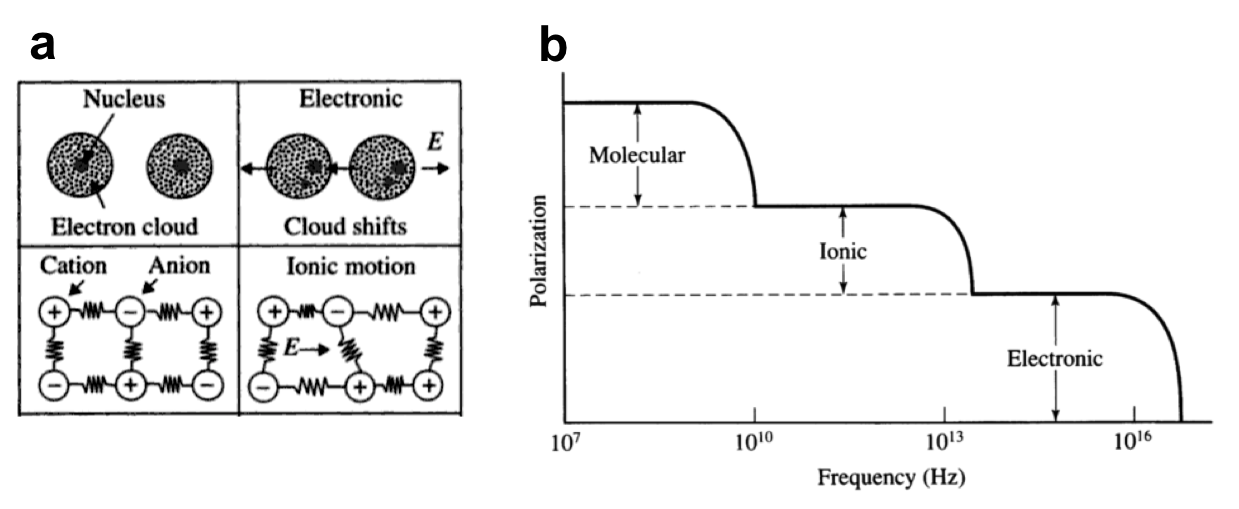
\includegraphics[width=0.9\textwidth]{figures/dielectric.png}
    \caption{Polarization mechanisms in a crystalline solid: response of electronic density and motion of ions (a), figure taken from \citenum{newnham}. Typical frequencies of applied electric field to induce polarization mechanisms, where the response at high frequencies is only that of the electronic density (b), figure adapted from reference \citenum{elec_prop_book}.}
  \label{dielectric}
\end{figure}

The value measured for the dielectric function for various frequencies of the applied electric field can give information about different dielectric responses of the material, some of which were shown in figure \ref{dielectric}. Furthermore, the dielectric function is usually a complex quantity, where the imaginary part corresponds a phase shift of the polarization relative to the applied electric field and leads to the attenuation, i.e. a gradual loss in the intensity, of electromagnetic waves as they pass through the material. The dielectric function is an important material property for a photovoltaic material for a number of reasons. Firstly, it can be shown that the absorption of a material, which has been discussed already as a way of comparing the performance of materials with direct and indirect band gaps in a solar cell, is mainly determined by the imaginary component of the dielectric function \cite{dielectric_func_book1}. The band gap determines the minimum energies photons must have in order to be absorbed by a material, but it does not predict how strongly that material will absorb them. 
In fact, it has even been suggested that when screening for candidate solar absorber materials, a direct band gap within the optimal range for the solar spectrum is not a sufficient criteria as this does not guarantee that the onset of absorption near the band gap is strong \cite{SLME}. In this particular work, instead of the Shockley-Quiesser limit mentioned earlier, they recommend an alternative screening metric, the Spectroscopic Limited Maximum Efficiency (SLME), which depends explicitly on the calculated absorption spectrum of the material.

\begin{figure}[h!]
  \centering
    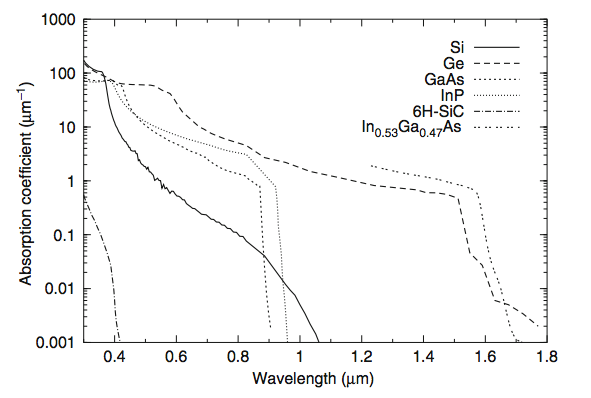
\includegraphics[width=0.9\textwidth]{figures/absorption_fig.png}
    \caption{Absorption coefficients of different semiconducting materials versus wavelength. Figure taken from reference \citenum{absorption_coeff_book1}.}
  \label{absorption_fig}
\end{figure}

\begin{figure}[h!]
  \centering
    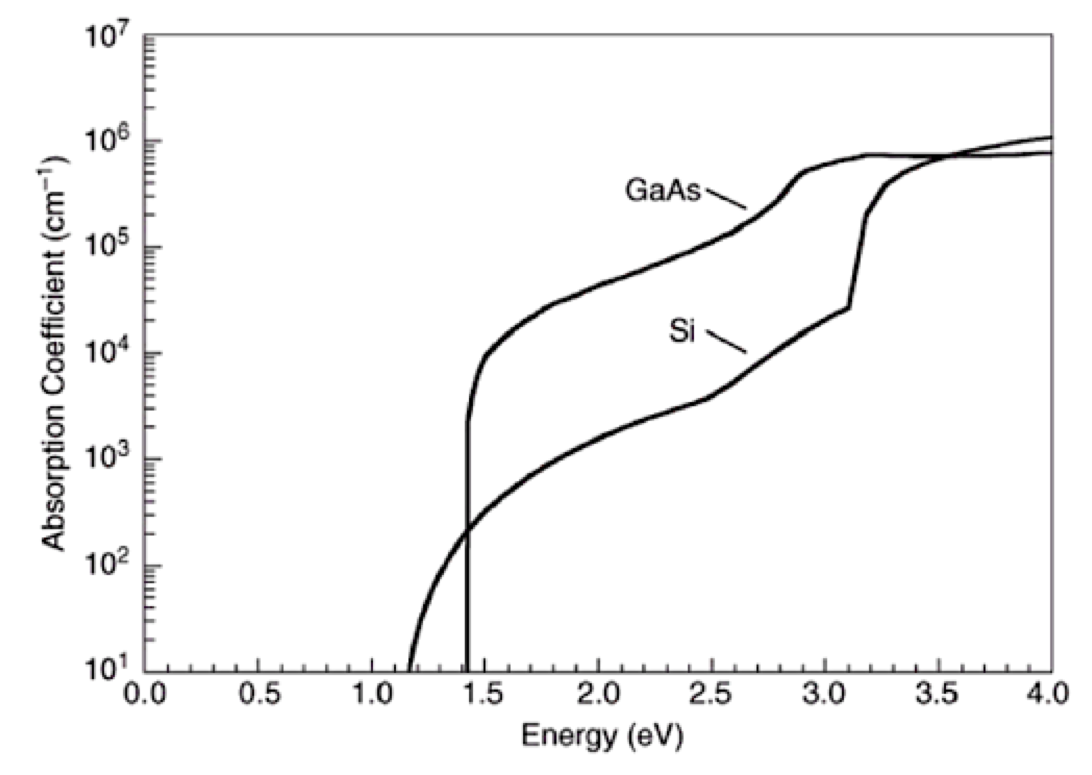
\includegraphics[width=0.9\textwidth]{figures/absorption_fig2.png}
    \caption{A comparison of the absorption coefficients of the indirect band gap semiconductor Si and the direct band gap semiconductor GaAs across a range of incident photon energies. Figure taken from reference \citenum{PV_bands_book}.}
  \label{absorption_fig2}
\end{figure}

The optical absorption coefficient of a material, $\alpha$, determines the penetration depth, $\frac{1}{\alpha}$, of light incident on the material \cite{absorption_coeff_book1}. Figure \ref{absorption_fig} shows the absorption coefficients of different semiconductors across a range of wavelengths. The figure shows a less steep onset of absorption for silicon, which as discussed earlier possesses an indirect band gap, compared to that of for example GaAs when the absorption corresponds to a direct band-to-band transition. The implication of the differing absorption coefficients and therefore different optical penetration depths of materials for solar devices is that materials which are stronger absorbers require less material to absorb the light. This forms the basis of thin-film solar cell technologies, for which the impact of defects in the absorber layer material are typically less significant as charge carriers do not have to travel through as much of the absorber material in order to reach a collection electrode. Different solar cell technologies will be discussed further in section \ref{current_tech}.

Secondly, the electrostatic force between an electron-hole pair is reduced when the static (or low-frequency) $\epsilon_r$ is larger \cite{dielectric_const1} due to the enhanced screening of the charge. This, therefore, will reduce the recombination of electron-hole pairs in a material. Another aspect of this property important for photovoltaic materials is that it can improve the defect tolerance of the material. In the majority of cases producing perfectly defect-free materials is impractical, if not impossible. The impact of defects in a material on photovoltaic performance will be discussed more in section \ref{defects_in_PV}, but for now it is just worth noting that defects can trap charge carriers, enhance electron-hole recombination (reducing carrier lifetimes in the material) and therefore have the overall effect of reducing charge collection from a PV device, thereby decreasing the efficiency of the conversion of incident photons into electrical current.
In reference to modelling electronic transport in a material in the presence of defects, $\epsilon_r$ has been referred to as the most important property of the material \cite{defect_tolerance}. A higher dielectric function indicates a greater ability to screen charge. The capture cross-section for charge carriers by a charged defect will therefore be influenced by the value of $\epsilon_r$ of the material \cite{defect_tolerance}. This property can therefore indicate how well photo-excited charge carriers will be transported through a defective photovoltaic material, towards an electrode for carrier collection and on to do electrical work.

\subsection{Current Commercial Solar Cell Technologies \& Limitations}\label{current_tech}
It was first observed in 1839 by Edmond Becquerel that sunlight could be used to generate electricity. Becquerel discovered that if  silver chloride was placed in an acidic solution, connected to platinum electrodes and exposed to sunlight, an electric current flowed. However the effect was small and poorly understood before Albert Einstein's discovery of the photoelectric effect and explanation of the phenomena by the quantum nature of light in 1904 \cite{PV_history1}. Even then, it was not until the development of semiconductor technology during the silicon revolution of the 1950's that solar cells were fabricated which were able to generate significant amounts of electricity. The first silicon solar cell was created in 1954 in the Bell Laboratories with cells achieving efficiencies of 6\%. 
Originally solar cells were developed for terrestrial energy generation, such as the 108 solar cells used to supply energy to the Vanguard satellite in 1958 \cite{PV_history1}. The first oil crisis in 1973 however highlighted the dependency of many economies on fossil fuels and the need to address the security of energy supply,  in particular for Japan and West Germany which had few of their own resources. As a consequence, solar cell research was no longer limited to only high-cost crystalline silicon devices for terrestrial applications, but also into creating cheaper, commercial, thin-film solar cell technologies using absorber materials such as amorphous silicon, cadmium telluride and copper indium diselenide  \cite{PV_history2}.\\

\begin{figure}[h!]
  \centering
    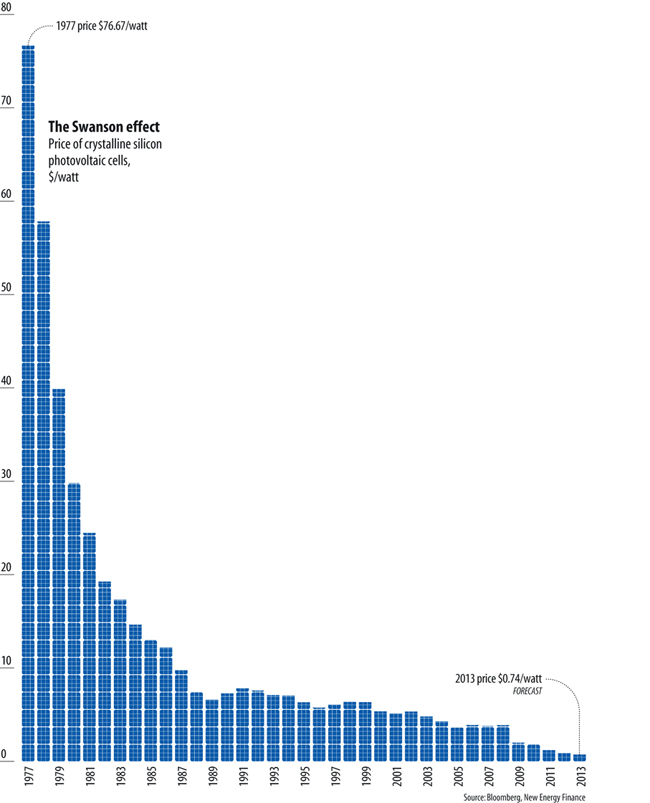
\includegraphics[width=0.7\textwidth]{figures/Si_cost.jpg}
    \caption{Average cost of solar panels composed of a crystalline silicon absorber layer. Figure taken from reference \citenum{PV_chart}.}
  \label{Si_cost}
\end{figure}

In spite of this, crystalline silicon is still the dominant solar cell technology with mono- and poly-crystalline silicon photovoltaic cells comprising up to 90\% of all the solar cells produced in 2008  \cite{Si_rev}. Silicon is the second most abundant element in the Earth's crust \cite{Si_abundance}, making it a plausible material to use in large-scale solar power generation. Over 60 years of development have seen device efficiencies increase from 6\% to 25\% for the highest quality research devices and 15-18\% for the more common industrial cells \cite{Si_rev}. As can be seen from figure \ref{SQ}, the best performing silicon devices are now very close to achieving conversion efficiencies close to their theoretical limit, as predicted by Shockley-Quiesser \cite{SQ_1961}. More dramatic however is the fall in manufacturing costs which have halved since 2008 and are more than a hundred times lower than they were in 1977, as shown in figure \ref{Si_cost}. This development was largely aided by progress in semiconductor technology driven by the silicon chip industry, with the solar industry benefiting from advances in silicon manufacturing processes and even making use of waste silicon produced that was not of a high enough grade for silicon chips \cite{PV_history1}. Although the development of silicon-based technologies has clearly revolutionized the modern computer, the optical properties of silicon do not make it ideal for use as a solar absorber material in a photovoltaic device and despite the dramatic reduction in manufacturing costs, the technology is still not able to be cost-competitive with fossil-fuel power generation, as was shown in figure \ref{LCOE}.\\

The primary issue with silicon is that its band gap of 1.1 eV is indirect. The key consequence of this property is that silicon is therefore not a very strong absorber of sunlight (compared to for instance newer, thin-film technologies which are discussed later), resulting in a low optical absorption coefficient  compared to these newer technologies where both band gap and absorption coefficient were two of the key material properties for solar cells discussed in section \ref{PV_properties}. To absorb the same amount of sunlight with a silicon solar cell requires a thicker layer of the material than in thin-film technologies. Photovoltaic devices are very sensitive to defects and impurities. This point is discussed further in section \ref{defects_in_PV}, but the consequence for a thick layer of silicon is that very high quality, non-defective material is necessary to enable charge carrier collection before recombination occurs, which results in high manufacturing costs. The devices are made from flat sheets of crystalline or multicrystalline silicon called wafers that consist of very high quality silicon (99.999999\% pure) 
\cite{sus_book_5}.
The production processes of silicon wafers have been thoroughly optimised, but are still very energy-intensive, time-consuming and complex \cite{emerging_pv} and this is reflected by the position of this type of technology on the plot of efficiency versus cost shown in figure \ref{PV_generations}. Despite decades of development, commercialized silicon solar panels are still too expensive to compete with fossil-fuel based power sources \cite{FE_PV_rev1_5}. \\

\begin{figure}[h!]
  \centering
    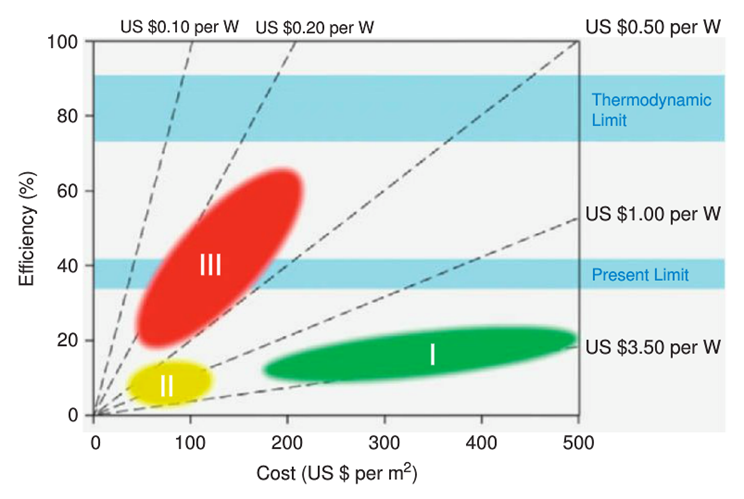
\includegraphics[width=0.75\textwidth]{figures/PV_generations.png}
    \caption{Efficiency and cost projections for first-, second- and third-generation photovoltaic technologies, which are comprised of silicon wafer, thin-film and advanced thin-film technology respectively. Figure 
 taken from reference \citenum{sus_book}.}
  \label{PV_generations}
\end{figure}

The `holy grail' of research into new materials for photovoltaic devices would be to find materials that are strong absorbers of sunlight that could also be produced cost-effectively from materials that are abundant enough for large-scale fabrication of the devices. Then it could be possible for solar energy generation to be economically viable on a large enough scale to replace fossil fuels to meet global energy needs. Such a drive has resulted in the development of what are considered three generations of solar energy technology. These are shown in figure \ref{PV_generations}, where highly efficient crystalline silicon devices with high associated manufacturing costs are considered the first generation of solar cell technology.
Thin-film solar cell devices are typically referred to as second-generation technology. These devices make use of materials that are much more optically thick than silicon (i.e. stronger absorbers of sunlight with higher optical absorption coefficients), which require less material to absorb the same amount of sunlight. It is then less important for the material to be of as high-quality as in crystalline silicon devices, which enables the use of low-cost and low-energy fabrication methods \cite{emerging_pv}. 
In the case of thin-film CuInSe$_2$ devices, it has even been found that the `lower quality' poly-crystalline material has a higher performance than its single crystal counterpart \cite{CIS1_3, CIS1_4}. Theoretical studies of the electronic properties of the grain boundaries in CuInSe$_2$ have provided an explanation for this unusual observation based on beneficial band offsets at the grain boundaries \cite{CIS1, CIS2}. This effect is a special case for this particular material, but it embodies the general ideology of thin-film technology well - namely to produce materials able to convert sunlight into electricity as efficiently as possible with the simplest synthesis techniques possible.
However typically the efficiencies of second-generation solar cells are less than that of the best performing first-generation devices. Examples of commercial thin-film technologies include CIGS (Cu(In,Ga)(S,Se)$_2$) and CdTe and figure \ref{SQ} shows that the best performing Si devices have higher efficiencies, which are also much closer to their theoretical limit, than these second-generation, thin-film technologies.
Third-generation PV technology aims to make use of the low cost fabrication techniques of the second-generation devices but use multiple energy threshold devices to overcome the Shockley-Quiesser limit for a single band gap solar cell, such as in tandem solar cells where semiconductor p-n junctions of increasing band gap are placed on top of each other in order to capture more of the solar spectrum. Typically the more complicated device architecture of third-generation devices result in higher fabrication costs. Research efforts are therefore largely focused on reducing the fabrication cost of multi-junction devices \cite{3rd_gen}.\\

Current mainstream solar cell technologies, such as first-generation Si wafers and second-generation thin-film CdTe and CIGS solar cells, would not be able to provide solar electricity at the terawatt scale due to the scarcity of Te and In and the relatively long energy payback time for crystalline Si due to the cost and energy intensive fabrication of Si wafers \cite{CZTS_vs_MAPI}. 
Models have even quantified such statements with a predicted In-constrained growth potential of power generation from CIGS PV technology of ~20 GW per year in 2020 due to competing applications of In, such as in liquid crystal displays \cite{culprit_5_3}.
In order to significantly increase the contribution of solar power to global power consumption, it is therefore necessary to develop more economically viable earth-abundant materials for sustainable PV electricity generation. Furthermore, there must be considerable technological breakthroughs that would enable low-cost manufacturing of highly efficient devices with enough of a cost benefit to outweigh the initial cost outlay in optimizing the manufacturing process of the whole device as has been done for silicon over the past 60 years. For this purpose, there is a drive for solar absorber materials with more optimal properties, such as a direct and sunlight matched band gap (as in thin-film technologies such as CdTe and CIGS), but also for materials that are composed of only earth-abundant components. 


\section{The Role of Computational Modelling in Material Design}
The discovery of new functional materials by experimental methods is largely hindered by high costs and time-consuming synthesis procedures \cite{high_tp}.
However, with the rapid increase in computational processing power and the availability of large-scale supercomputers, we are entering a very exciting era in computational materials design. 
There are two main contributions that computational simulations could make towards the technological breakthroughs needed for the development of photovoltaic devices for economically-viable, large-scale solar energy generation. Firstly by predicting properties and screening for certain desirable properties for a solar absorber material, such as an optimal band gap and high carrier mobility, materials simulations are able to aid in the discovery of new materials for use in photovoltaic devices. Secondly, material simulations are able to provide valuable insight to improve understanding of known photovoltaic materials to enable the synthesis of better performing devices. So far in this study we have aimed to make both of these contributions to the field. Firstly, we perform simulations to understand the performance bottlenecks in the candidate earth-abundant, non-toxic solar absorber material \CZTS (CZTS) and we also study the optical properties of three candidate photovoltaic materials which have so far received little attention as solar materials but could provide another possible route for high-performance photovoltaic devices for cost-effective solar energy generation.


\section{Overview of this Study}

\subsection{Promising Candidate Solar Absorber Materials}
Refer to: CH 5 (other PV materials) + pg 187 (future of PV) \cite{PV_Goetzberger}\\

As already discussed, to make solar energy generation on a large scale economically viable, it must be possible to make devices with an LCOE that is comparable to fossil-fuel resources. Furthermore, the materials that make up the devices must also be sufficiently abundant such that there would be enough to make a substantial number of devices in the first place. For this reason there is a drive for photovoltaic materials that could be made using the lost-cost methods associated with second-generation technology, but containing only earth-abundant components. Gauging the abundance of a given material is not as trivial a process as looking at crustal abundance as supply, demand, geographical distribution and extraction must all be considered. However, knowledge of solar cell technologies made from various different materials opens up the possibility of utilizing multiple different materials to collectively contribute to the global solar power capacity to enable larger-scale power generation from this renewable, low-carbon resource. Additionally by studying various different materials, the scientific community could eventually discover a select few that have the best properties to enable low-cost synthesis of highly efficient devices to eventually significantly reduce the LCOE of solar power.\\

Presently, two of the most studied candidate earth-abundant thin-film solar cell materials include Cu$_2$ZnSnS$_4$ (CZTS) and methylammonium lead iodide (CH$_3$NH$_3$PbI$_3$ or MAPbI$_3$) \cite{CZTS_vs_MAPI}. The potential of CZTS for photovoltaic applications was realised in 1988 by Ito and Nakazawa \cite{first_CZTS}. The band gap of the material has been predicted \cite{CZTS_bandgap_theory} and measured \cite{CZTS_bandgap_exp} to be 1.5 eV, which corresponds to a theoretical conversion efficiency limit of 28\% as predicted by Shockley-Quiesser \cite{SQ_1961}. However, the current record device efficiency is 8.8\% \cite{CZTS_record} and it is believed that this figure must be increased to at least 15\% for the devices to be commercially viable \cite{SS}. PV devices composed of a CZTS absorber layer are hampered by low open circuit voltage (V$_{OC}$) \cite{SS}, which is believed to be due to the formation of secondary phases \cite{CZTS_phases} and defects \cite{CZTS_defects} in CZTS, although the exact origin of the low V$_{OC}$ remains unknown. The first component of this study is therefore an attempt to determine possible origins of this deficit in CZTS.\\

MAPbI$_3$ is an example of a hybrid halide perovskite solar cell material, which are regarded as a convergence of inorganic thin-film and dye-sensitised solar cells (DSSC's) \cite{Federico}. Research on such materials dates back to 1928 \cite{Jarv_7}. The efficiency of MAPbI$_3$ solar cells however has increased rapidly between 2009 and 2014 from 3.8\% for MAPbI$_3$-based DSSC's to 20.1\% for a planar MAPbI$_3$-based thin-film solar cells \cite{CZTS_vs_MAPI} and has therefore surpassed the record efficiency of both conventional DSSC's as well as the earth-abundant thin-film PV absorber material CZTS \cite{Federico}. Electricity generation in a typical PV device, such as that shown in the schematic in figure \ref{PV_schematic}, is dependent upon charge separation by variation in material composition, as in a p-n junction. However, in ferroelectric materials charge separation can also be achieved due to the intrinsic crystal field in a homogeneous material. The crystal polarity creates microscopic electric fields across domains, separating photogenerated excitons into free charges, and segregating the transport of the free charges to reduce recombination rates \cite{keith}. Hybrid perovskites have been shown to exhibit spontaneous electric polarization \cite{Jarv}.
Therefore, one possible explanation for the high efficiency of MAPbI$_3$-based solar cells is enhanced separation of photoexcited electron and hole pairs, and hence reduced rate of electron-hole recombination, due to the presence of ferroelectric domains \cite{Jarv, Federico}. Although the stability of MAPbI$_3$-based solar cells has been identified as a big challenge for these devices, as CH$_3$NH$_3$PbI$_3$ is very sensitive to polar solvents such as water and so readily dissolves and decomposes into PbI$_2$ \cite{MAPI}. \\

A number of interesting PV phenomena have been observed in ferroelectric (FE) materials  such as the bulk photovoltaic effect (BPE) and the anomalous photovoltaic effect (APE) \cite{keith}. Ferroelectric materials usually have a high dielectric constant (which was mentioned in section \ref{PV_properties} as an important parameter for a photovoltaic material) and they possess a spontaneous electric polarization that can be switched between two or more states using an electric field \cite{new_FE_PV_1}.
The BPE was first recorded in 1956 in BaTiO$_3$ \cite{keith_46}, where photovoltages were measured in un-doped single crystals \cite{keith}.
The BPE effect is distinctly different from the typical PV effect in semiconductor
p-n junctions as it is the polarization electric field that is the driving force for the photocurrent in FE-PV devices \cite{FE_PV_rev1}. 
The APE was first observed in PbS films in 1946 \cite{keith_54} and has since been reported in polycrystalline CdTe, ZnTe, InP \cite{keith_55, keith_56, keith_57}, where photovoltages output along the polarization direction can be significantly larger than the band gap of the material \cite{FE_PV_rev1}, which is usually the limit for a semiconductor PV material \cite{keith}. 
The Shockley-Queisser limit, which prevents any single p-n junction solar cell from converting more than 33.7\% of the incident light into electricity, has not been predicted to apply for these photovoltaic phenomena. An upper limit for the theoretical power conversion efficiency (PCE) from this photovoltaic mechanism seems to still be an open question \cite{new_FE_PV}, although an ultimate maximum efficiency of any single-band gap absorber of 44\% has been set by thermodynamic considerations \cite{SQ_1961}. Theories to explain the PV phenomena observed in FE materials are discussed further in section \ref{FE_PV_section}.\\

The identification and understanding of such phenomena may open up the possibility of more efficient PV devices constructed from a number of different photoferroelectric materials. However, most of the commonly used ferroelectric materials such as LiNbO$_3$ and BaTiO$_3$ have band gaps larger than 3 eV and can therefore only absorb sunlight in the UV range to convert into electricity, which accounts for only around 3.5\% of the solar spectrum \cite{FE_PV_rev1}, which is illustrated in figure \ref{solar_spectrum}. The optimal range for the band gap in order to absorb the majority of the solar spectrum under typical radiation conditions is between 1.06 eV and 1.50 eV \cite{CZTS_book}. Research efforts have also gone into adjusting the optical absorption of ferroelectric materials without influencing the ferroelectric properties of the material through chemical doping or alloying \cite{FE_PV_rev1}. In Bi$_4$Ti$_3$O$_{12}$ (BiT) the optical band gap has been tuned in such a way, resulting in a decrease from 3.6 eV to 2.7 eV \cite{FE_PV_rev1_83}, although this is still considerably larger than the optimal range for a PV absorber material.\\

This then leads on to the second component of this study, which is an investigation of the optoelectronic properties of new candidate solar absorber materials that may also exhibit ferroelectricity, but have band gaps within the optimal range for the absorption of sunlight. In theory, these materials may exhibit the exceptionally high performance of MAPbI$_3$-based solar cells (ideally without the instability issues suffered by MAPbI$_3$) or enable the possibility of exploiting other novel photovoltaic phenomena such as the anomalous and bulk photovoltaic effects to overcome the Shockley-Quiesser efficiency limit without the need for such complicated device architectures as in third-generation tandem solar cells. Although the difference between the Shockley-Quiesser limit and the ultimate thermodynamic limit of a solar material is not enormous, it is also possible that ferroelectric materials have properties that enable more efficient devices to be made more easily, such as good screening of the effect of defects due to a high dielectric constant or enhanced electron-hole separation from ferroelectric domains resulting in reduced recombination and a higher performance solar cell with `low quality' defective and nanostructured materials. Such technologies could provide one possible route for the technological breakthrough that could enable economically-viable, large-scale solar energy generation.

\subsection{Investigating Possible Performance Bottlenecks of {\CZTS } Devices}
** Check against Laurie's April highlights (top two bullet points on disorder)\\

\begin{figure}[h!]
  \centering
    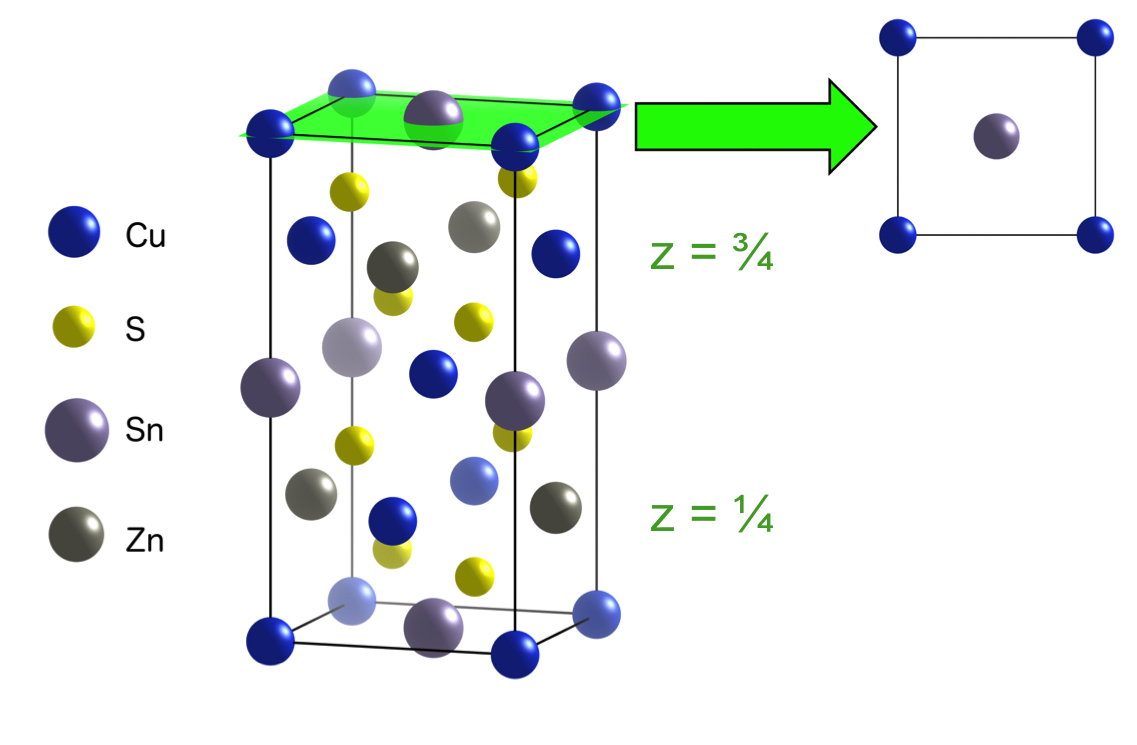
\includegraphics[width=0.7\textwidth]{figures/CZTS_cell.png}
    \caption{The conventional unit cell of CZTS (Cu$_{2}$ZnSnS$_{4}$) with the ground-state kesterite crystal structure (space group $I\bar{4}$). The structure consists of alternating layers of Cu-Sn and Cu-Zn where Cu-Zn layers are at z=$\frac{1}{4}$ and z=$\frac{3}{4}$.}
  \label{CZTS_cell}
\end{figure}

The ground state crystal structure of CZTS (Cu$_{2}$ZnSnS$_{4}$) is kesterite (space group $I\bar{4}$). The conventional unit cell of CZTS is shown in figure \ref{CZTS_cell}, where each S is surrounded by two Cu, one Zn, and one Sn to satisfy local charge neutrality and the valence-octet rule.
Kesterites meet two necessary conditions for highly efficient solar cells, which are a band gap that is both direct and relatively well-matched to the solar spectrum \cite{CZTS_book}.
Over the last decade the power conversion efficiency of PV devices based on kesterite, Cu$_2$ZnSn(S$_x$Se$_{1-x}$)$_4$ (CZTSSe), compounds has improved greatly from around 5\% in 2004 to 12.6\% in 2013 \cite{culprit_2}. However, this is still far from the record efficiencies of Cu(In$_{1-y}$,Ga$_y$)Se$_2$ (CIGSe) devices of $>$20\%, where the materials have very similar band gaps to those of CZTSSe \cite{culprit} and so should have the same theoretical efficiency limit as predicted by Shockley and Queisser \cite{SQ_1961}. Furthermore, the rate of improvement seems to have slowed considerably recently with the last improvement in efficiency being reported in 2014 and with only a 0.1\% improvement \cite{culprit_3}. A large number of possible explanations have been proposed to explain the current difference in efficiency between CZTSSe and CIGSe devices, many of these are illustrated in figure \ref{kesterite_bottlenecks}. The majority of studies converge towards the low open circuit voltage (V$_{OC}$) relative to the band gap, i.e. the V$_{OC}$ deficit, being the main limiting factor on device performance. As can be seen from the position of CZTSSe devices on the plot in figure \ref{Voc}, the open circuit voltages measured for these devices are considerably less than that of a CIGS device, which has a similar value for the band gap of the material.\\

\begin{figure}[h!]
  \centering
    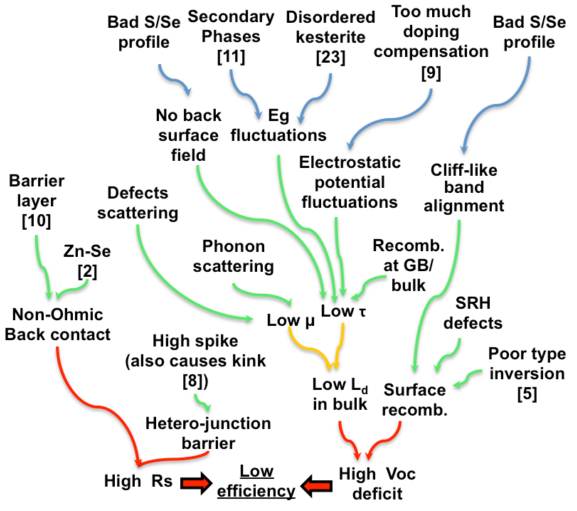
\includegraphics[width=0.75\textwidth]{figures/kesterite_bottlenecks.png}
    \caption{Mapping of the numerous possible mechanisms limiting the efficiency in kesterite devices and their possible causes. R$_s$ is the series resistance between the absorber layer and back contact of the device and V$_{OC}$ is the open circuit voltage across the absorber layer. Figure take from \citenum{CZTS_scale_up}.}
  \label{kesterite_bottlenecks}
\end{figure}

\begin{figure}[h!]
  \centering
    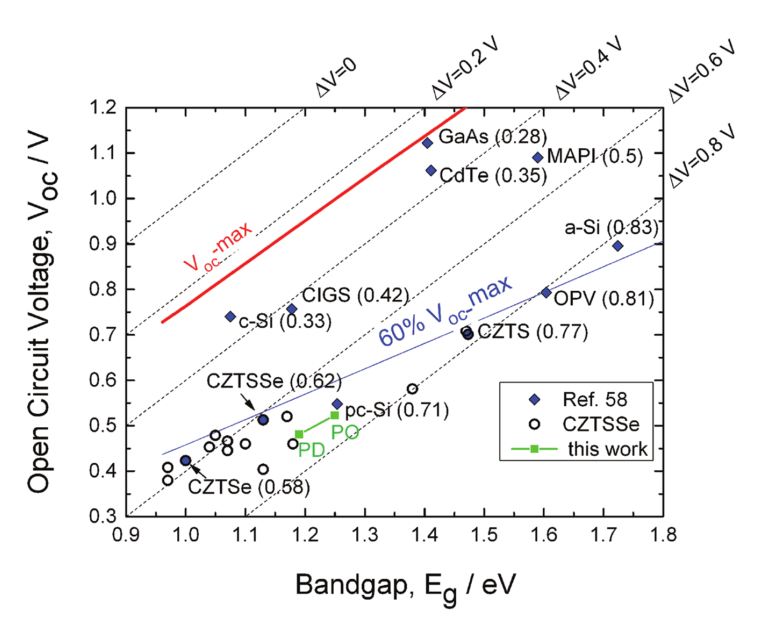
\includegraphics[width=0.85\textwidth]{figures/Voc.png}
    \caption{V$_{OC}$ versus band gap of high performance CZTSSe devices ($>$9\% efficiency) indicated by circles with best devices based on other photovoltaic materials shown for comparison by diamond symbols: Methyl-ammonium lead iodide (MAPI), amorphous silicon (a-Si), organic photovoltaic films (OPV), crystalline silicon (c-Si) and polycrystalline silicon (pc-Si). The oblique lines give a constant V$_{OC}$ deficit from 0.8 V to 0 V. The green points correspond to CZTSSe films that are partially ordered (PO) or partially disordered (PD) due to disorder amongst Cu and Zn. Figure take from reference \citenum{culprit}.}
  \label{Voc}
\end{figure}

As figure \ref{kesterite_bottlenecks} shows, there are many different possible causes of the  V$_{OC}$ deficit in kesterite solar cells. Developing fabrication techniques to reduce the deficit is therefore an even greater challenge when the exact cause is not yet known.
This is an area in which computational materials simulations should be able to provide valuable insight to help pinpoint the specific sources of the V$_{OC}$ deficit in kesterite solar cells. The true power of simulation is the ability to take a perfect system and introduce various imperfections one and a time and then study the effect that particular imperfection could have on device performance. As opposed to in a real system in which there is a myriad of possible causes for each observation, as illustrated in figure \ref{kesterite_bottlenecks}.
In our simulations we will start from the most simple system possible, before making any attempts to build up in complexity. Devices made from a compound of \CZTS  and Cu$_2$ZnSnSe$_4$, i.e. Cu$_2$ZnSn(S$_x$Se$_{1-x}$)$_4$, so far have given the highest performance devices, however in this study we are currently focusing on just the pure selenide material, CZTS. In addition to simplifying the system, figure \ref{Voc} also indicates that the V$_{OC}$ deficit is worse in purely CZTS devices and so potentially studying causes of the problem in this particular system could be more informative. Also although ultimately the aim is to make thin-film devices from CZTS, in which the material is likely to be highly polycrystalline with many grain boundaries, we are currently just focusing on the bulk material. We are doing this for two reasons. Firstly to improve the understanding of the fundamental material properties before attempting to understand a more complex system to ensure we start from a solid foundation. Secondly, it has been proposed that the V$_{OC}$ deficit in CZTSSe devices could actually be largely due to the natural bulk properties of the crystal \cite{culprit_5}. For the purposes of our study therefore measurements performed on single crystals will be the most directly relatable to our findings, wherever the data is available.\\

\begin{figure}[h!]
  \centering
    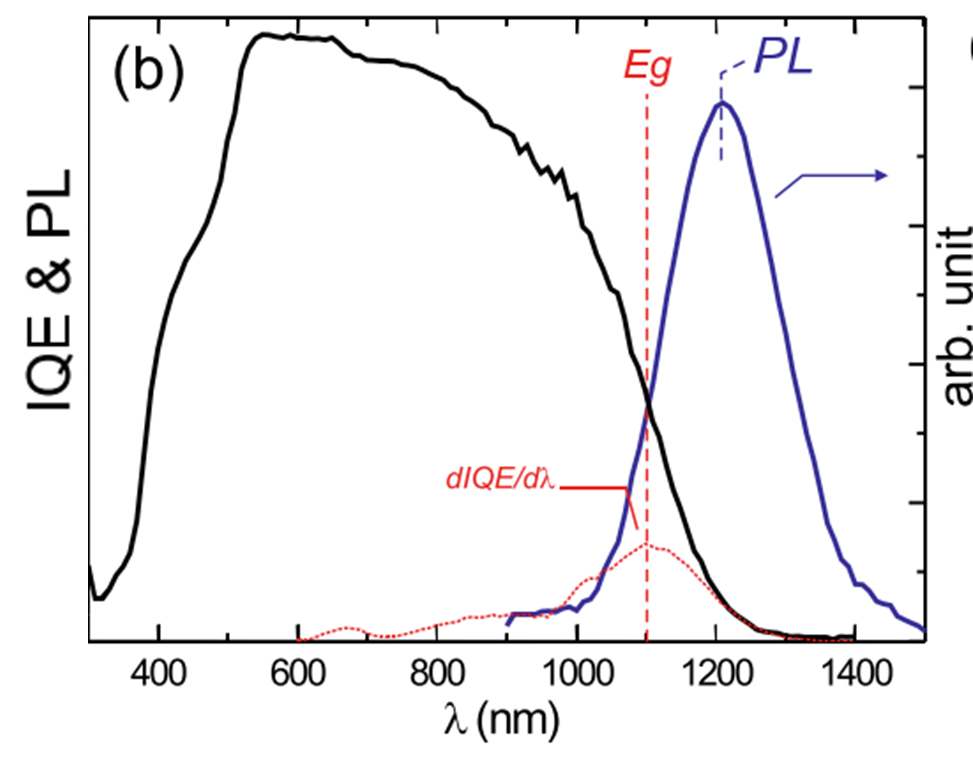
\includegraphics[width=0.7\textwidth]{figures/CZTS_PL.png}
    \caption{Internal quantum efficiency (IQE) and photoluminescence (PL) spectra of CZTSSe thin-films showing the shift of the PL peak to energies below the band gap of the material. Figure take from reference \citenum{band_tail}.}
  \label{CZTS_PL}
\end{figure}

\begin{figure}[h!]
  \centering
    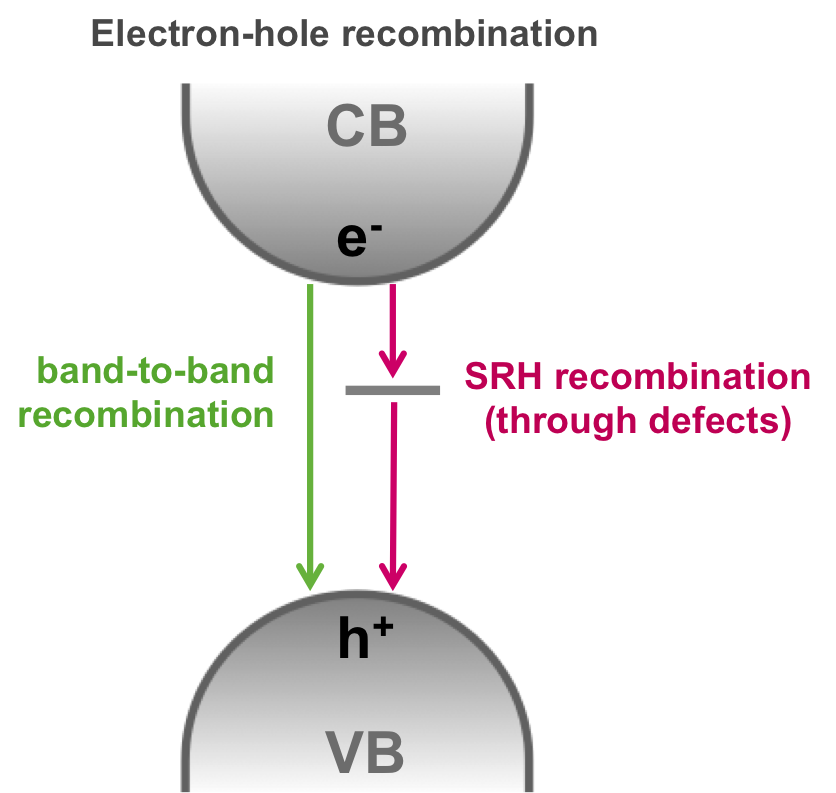
\includegraphics[width=0.45\textwidth]{figures/SRH.png}
    \caption{Illustration of Shockley-Read-Hall (SRH) electron-hole recombination due to energy states introduced into the band gap by defects.}
  \label{SRH}
\end{figure}

In general, the main cause of V$_{OC}$ deficit in a PV device is the recombination of photogenerated charge carriers in the bulk material or at surfaces \cite{culprit}. 
Figure \ref{CZTS_PL} shows photoluminescence (PL) spectroscopy measurements performed on CZTSSe thin films by Gokmen et al \cite{band_tail}. The emission spectra of semiconductors is discussed much more thoroughly in section \ref{PL_section} and a review of various PL studies performed on kesterite thin films and crystals is given in section \ref{CZTS_PL_section}, but for current purposes the key observation to be made from figure \ref{CZTS_PL} is that there is a shift in the PL peak to lower energies (red-shifting), below the value of the band gap obtained from internal quantum efficiency (IQE) measurements performed on the same thin films. It is also noted in this study when comparing the PL spectra of CZTSSe films to that of CIGSSe films that the PL peak for CZTSSe thin films is broader and that the red-shifting was roughly twice as severe. This effect is referred to as `band-edge tailing', where photons of energies less than the band gap of the material are emitted following photoexcitation and subsequent relaxation back to the ground state. This effect is known to be detrimental for device performance as emitted photons may then not have sufficient energy for subsequent photoexcitations in the absorber layer, the energy of the original photon may then not be converted into electricity if the photoexcited electron-hole pair recombine before the charge is collected \cite{Nelson4}. Band tailing and the possible causes of this detrimental effect are discussed further in section \ref{defects_in_PV}, but for now it is worth briefly noting that possible causes are: Shockley-Read-Hall recombination due to defect-induced mid-gap states \cite{SRH}, as illustrated in figure \ref{SRH}, as well as fluctuations in electrostatic potential due to the presence of charged defects and fluctuations in the band gap of the material due to an inhomogeneous composition \cite{band_tail}, which are both shown in figure \ref{band_tail_fig}.\\

\begin{figure}[h!]
  \centering
    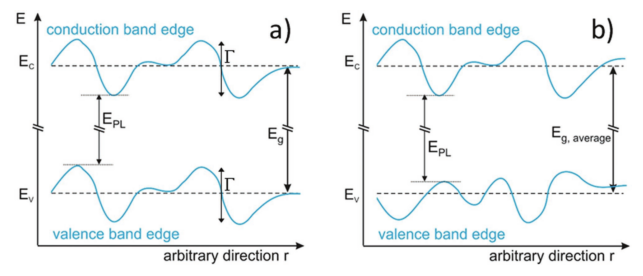
\includegraphics[width=0.9\textwidth]{figures/band_tail_fig.png}
    \caption{The effect of electrostatic potential fluctuations (a) and band gap fluctuations (b) on the electronic bands of a semiconductor. In both cases radiative transitions at energies below the (average) band gap are possible. The band gap in a is constant and not affected by local charged defects, while band edges in b can differ depending on e.g., long range composition variations. Figure taken from reference \citenum{culprit}.}
  \label{band_tail_fig}
\end{figure}

The extent of band tailing due to the additional energy levels introduced into the band gap of a material by particular intrinsic defects is dependent upon the concentration of those particular defects. The equilibrium defect concentration can be obtained directly from the defect formation energy \cite{DFT_in_mat}, which is discussed further in section \ref{defect_sections}. For materials such as CZTSSe that are still at a fairly early stage of development, theoretical predictions of defect formation energies may be the only values available to help identify specific defects and their properties in real systems \cite{kosyak}. Theoretical predictions for the formation energies and depth of defect-induced energy levels for various intrinsic point defects and defect clusters in CZTS made by Chen et al \cite{defect1} are shown in figures \ref{Chen_pt1}, \ref{Chen_pt2}, \ref{Chen_cluster1} and \ref{Chen_cluster2}. Based on the predictions made by Chen et al, figure \ref{Chen_pt2} shows that many of the intrinsic defects involving Sn would induce a mid-gap state, however figure \ref{Chen_pt1} shows that the formation energy of those particular defects would all be expected to be high. It therefore would be expected that these defects are less likely to form and should be present in lower concentrations than other defects. Although other works have suggested that the formation of this defect could be more likely if it is forms part of a particular defect cluster \cite{CZTS_n-type, culprit}. From the work by Chen on defect clusters, it is also expected that certain charge compensated defect clusters would have very low formation energies, in particular the $[Cu_{Zn}^{-} + Zn_{Cu}^{+}]$ antisite defect pair, as shown in figure \ref{Chen_cluster1}.\\

Disorder amongst Cu and Zn ions (or equivalently the formation of the $[Cu_{Zn}^{-} + Zn_{Cu}^{+}]$ antisite defect pair) in CZTS has been proposed as one possible origin of the V$_{OC}$ deficit in CZTS and consequently a number of experimental studies have been conducted to investigate this \cite{Scragg, pot_fluc_4, neutron, Schorr}. Additionally it is worth noting that this substitutional disorder does not exist in the crystal structure of CIGSe due to the considerably larger chemical mismatch between Cu with In or Ga \cite{culprit}, whereas Cu and Zn are so similar that disorder between the two species can be difficult to detect experimentally. 
As Cu and Zn are neighbouring elements in the periodic table, the changes in the bonding between the two are subtle \cite{pot_fluc}. This results in a theoretical energy difference between the two structures of just 3 meV per atom \cite{Chen2009} allowing for intermixing of the Cu and Zn cations in CZTS, which has been confirmed by neutron diffraction \cite{pot_fluc_4, neutron} and also measured using near resonant raman scattering \cite{Scragg}. However, a recent work prepared samples with varying degrees of Cu-Zn disorder (by varying the cooling rate during synthesis, which had been shown in a previous study to have a considerable effect on Cu-Zn ordering in CZTS \cite{Scragg}) and in this work they showed that a reduction in Cu-Zn order resulted in a reduction in both the band gap and V$_{OC}$, thereby not influencing the V$_{OC}$ deficit relative to the band gap of the material \cite{culprit}.

\begin{figure}[h!]
  \centering
    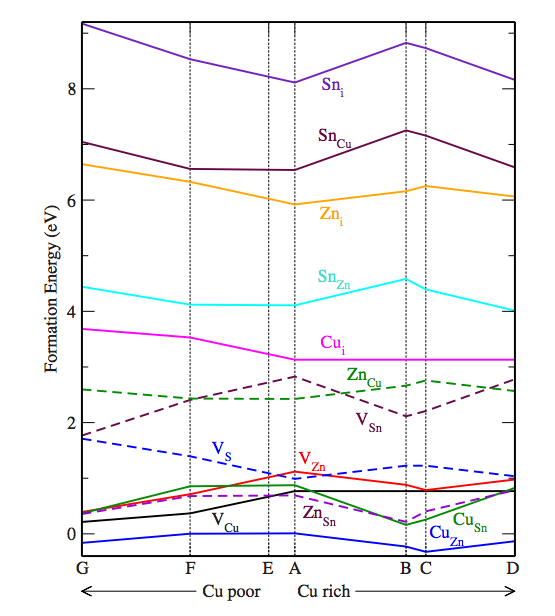
\includegraphics[width=0.8\textwidth]{figures/Chen_pt_formE.png}
    \caption{The formation energy of neutral intrinsic defects in \CZTS as a function of the chemical potential. Figure taken from reference \citenum{defect1}.}
  \label{Chen_pt1}
\end{figure}

\begin{figure}[h!]
  \centering
    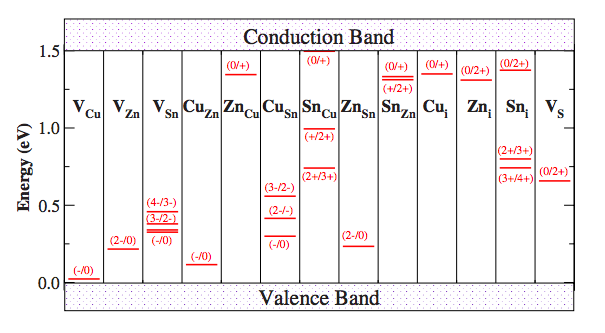
\includegraphics[width=0.8\textwidth]{figures/Chen_pt_E-level.png}
    \caption{The transition-energy levels of intrinsic defects in the band gap of \CZTS where the GGA band gap has been corrected to the experimental value 1.5 eV, and the donor levels are shifted together with the conduction band minimum (CBM) level. Figure taken from reference \citenum{defect1}.}
  \label{Chen_pt2}
\end{figure}

\begin{figure}[h!]
  \centering
    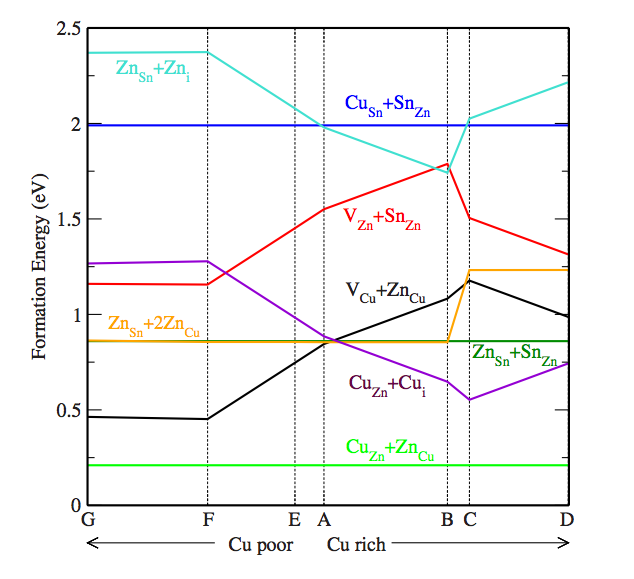
\includegraphics[width=0.8\textwidth]{figures/Chen_cluster_formE.png}
    \caption{The formation energy of charge compensated defect complexes in \CZTS as a function of the chemical potential. Figure taken from reference \citenum{defect1}.}
  \label{Chen_cluster1}
\end{figure}

\begin{figure}[h!]
  \centering
    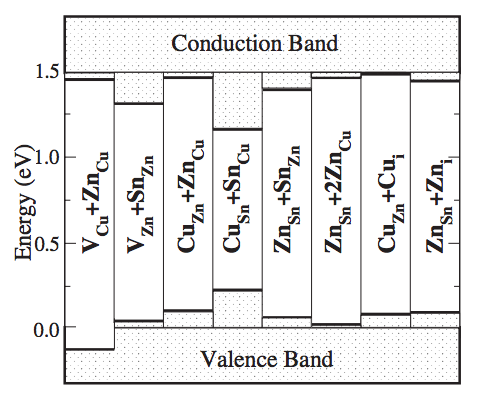
\includegraphics[width=0.7\textwidth]{figures/Chen_cluster_E-level.png}
    \caption{The conduction band minimum (CBM) and valence band maximum (VBM) levels in eV of \CZTS with different charge-compensated defect complexes relative to the host material at 0 eV and 1.5 eV respectively. Figure taken from reference \citenum{defect1}. }
  \label{Chen_cluster2}
\end{figure}

In this work we begin three investigations to explore some of the possible explanations for the V$_{OC}$ deficit in CZTS solar cells and to attempt to explain the PL spectra of CZTS shown in figure \ref{CZTS_PL}. 
As discussed above, intrinsic defects can introduce additional energy levels into the band gap of the material and energy states within the band gap are Shockley-Read-Hall recombination sites \cite{SRH}.
We re-investigate the formation energy of sulfur vacancies (V$_S$) in CZTS. This is another possible deep donor defect in CZTS and it was proposed in a recent study using admittance spectroscopy measurements performed on CZTSSe, combined with electrical modelling, that in addition to majority p-type defects in CZTSSe (giving the material its p-type conductivity), there may also been deep n-types defects \cite{CZTS_n-type}.
V$_S$ in CZTS has been predicted to produce a mid-gap state in the band gap of the material \cite{defect1}, which could provide one explanation for the poor device performance. However in the same work this particular point defect was also predicted to have a high formation energy relative to other possible intrinsic defects, making it less likely to form. However, it is possible that the formation energy of this defect is reduced when considering the typical annealing conditions of CZTS in which S is in the gaseous phase. We therefore calculate the formation energy of a V$_S$ in CZTS as a function of the sulfur chemical potential, which has been calculated as a function of temperature and pressure in a previous study \cite{Adam_sulfur}, making it possible for us to compare directly to experimental synthesis conditions.\\

Secondly, we examine possible causes of band gap broadening, which has been observed in electromodulation (??) measurements performed on CZTS crystals \cite{PVTEAM_paper}. We use materials modelling to determine the intrinsic band gap broadening to be expected even in perfect, bulk CZTS due to thermal lattice expansions. This contribution can then be subtracted from band gap broadening measured experimentally to determine how much of this effect is due to disorder and other factors. 
Lastly, we simulate thermodynamic substitution amongst Cu and Zn ions in CZTS and study the resulting changes in the distribution of electrostatic potential in the system in an attempt to extract the contribution of this particular type of disorder to the strong band tailing that has been observed in kesterite devices, which has been suggested to be due to fluctuations in electrostatic potential \cite{band_tail}.
As discussed above, disorder amongst Cu and Zn ions has not only be predicted to be very likely based on energetics but has also been observed experimentally, it would therefore be important to know if this particular type of disorder is having a detrimental effect on device performance or to at least eliminate it from the list of many possible causes of the V$_{OC}$ deficit.\\
**Edit last paragraph once PVTEAM paper published so have more info + put eris study first to match order of results?**
 


\subsection{Predicting the Properties of New Candidate Solar Absorber Materials}
The second part of this study involves using materials modelling to predict the optoelectronic properties of materials that could have the potential to be used to produce high performance PV devices, but until now have received little research interest for applications in PV.  The central idea in selecting these candidate materials was to identify any that may be ferroelectric and so could exhibit some of the novel FE-PV phenomena discussed earlier but may also have a band gap within the optimal range for solar absorption. Photoferroelectric, or photoferroic, is the name given to materials that exhibit such properties. 
Using very simple screening criteria, we identified three candidate photoferroelectric solar absorber materials from a data set of over 200 naturally occurring minerals. 
A dark-coloured material suggests (but does not guarantee) that it absorbs light in the visible range. Ferroelectric materials are a subset of materials with polar crystal structures, therefore not all polar materials exhibit ferroelectricity. It is only polar materials that also possess a spontaneous electric dipole moment within the unit cell which can be inverted by the application of an external electric field that exhibit ferroelectricity \cite{FE_subset}. 
Therefore, the conditions used to screen for candidate photoferroelectric materials shown in the Venn diagram in figure \ref{vd} are necessary conditions for photoferroelectricity, but cannot guarantee this property as a polar space group is a necessary but not sufficient condition for ferroelectricity.
The three candidate photoferroelectric materials identified by our screening process were: enargite (\enargite), stephanite (\stephanite) and bournonite (\bournonite). All three minerals are sulfosalts, which are materials that contain two or more metals, semi-metals such as antimony and arsenic, and sulfur \cite{DK}. \\

\begin{figure}[h!]
  \centering
    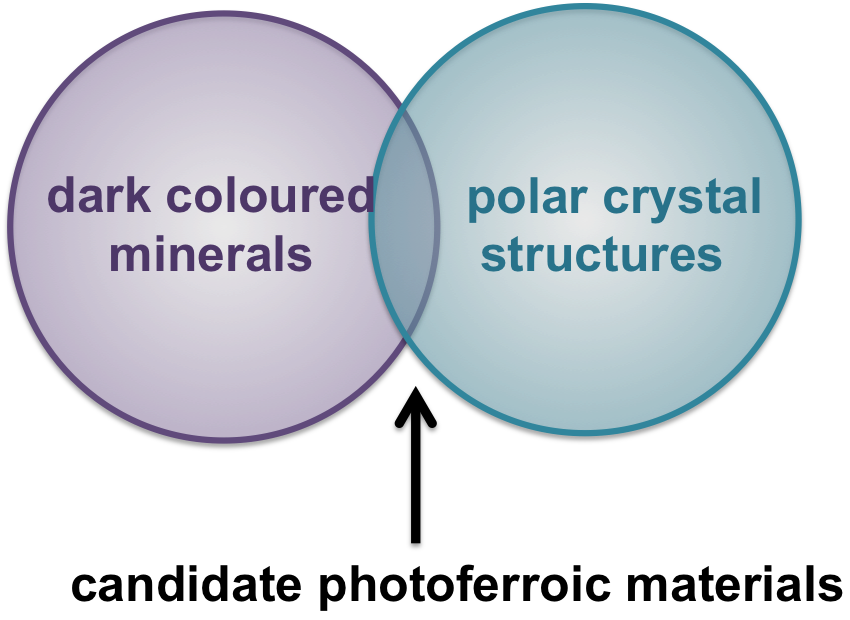
\includegraphics[width=0.5\textwidth]{figures/venn_diagram.png}
    \caption{Venn diagram showing the necessary (but not sufficient) conditions for a material to exhibit photoferroelectricity, where the dark colour suggests absorption of light in the visible range and a polar crystal structure is a requirement (but does not serve as a guarantee) for a material to exhibit ferroelectricity.}
  \label{vd}
\end{figure}

Scientific research on sulfosalts has largely focussed on the thermodynamic properties and crystal structure of the materials, leaving knowledge of the optoelectronic properties of sulfosalts relevant for PV applications extremely scarce. 
The potential of sulfosalt minerals for PV applications however was highlighted by Dittrich et al in 2007 \cite{Dittrich2}. This work also provides an overview of thin film deposition methods that have been developed for sulfosalt layers and discusses a 1\% efficient Sn-Sb-S sulfosalt thin film solar cell constructed by the authors. The thin film deposition methods discussed for other sulfosalt materials would also be particularly important for the eventual aim of constructing PV devices from these materials. The potential of the sulfosalt mineral enargite for PV applications has been suggested even earlier by Pauport\'{e} and Lincot in 1995 \cite{enargite_properties}. In addition to synthesis methods, another important consideration for the large-scale deployment of solar devices composed of the candidate materials is the price and abundance of the elemental components. Figure \ref{abundance} shows a comparison of the price and abundance of some of the elemental components of the three candidate materials: Cu, Sb and S, to that of elements used in some current commercial thin film solar cell absorber materials such as CuIn(Ga)Se$_{2}$ (CIGS) and CdTe. The components of the candidate materials not included in the figure are As, Pb and Ag. Lead can be considered as the most abundant and universally diffused metal after iron. Although it is never found in the native state, its ores are very numerous \cite{abundance}. 5,200,000 tonnes of lead was produced in 2012 \cite{ab_prod}, although its crustal abundance is considerably smaller than that of iron being around 10-14 ppm to compared to approximately 60,000 ppm for iron \cite{ab_1}. 
Silver and arsenic are both fairly abundant metals. Silver often occurs in combination with lead, copper, iron, antimony and tellurium. Arsenic is also present in most ores of silver \cite{abundance}. The crustal abundance of arsenic is approximately 1.5 ppm and that of silver is relatively low at approximately 0.070 ppm \cite{ab_1}. These values are however still larger than that of indium (0.049 ppm \cite{ab_1}), which is also in demand for the display industry \cite{SS}.\\

\begin{figure}[h!]
  \centering
    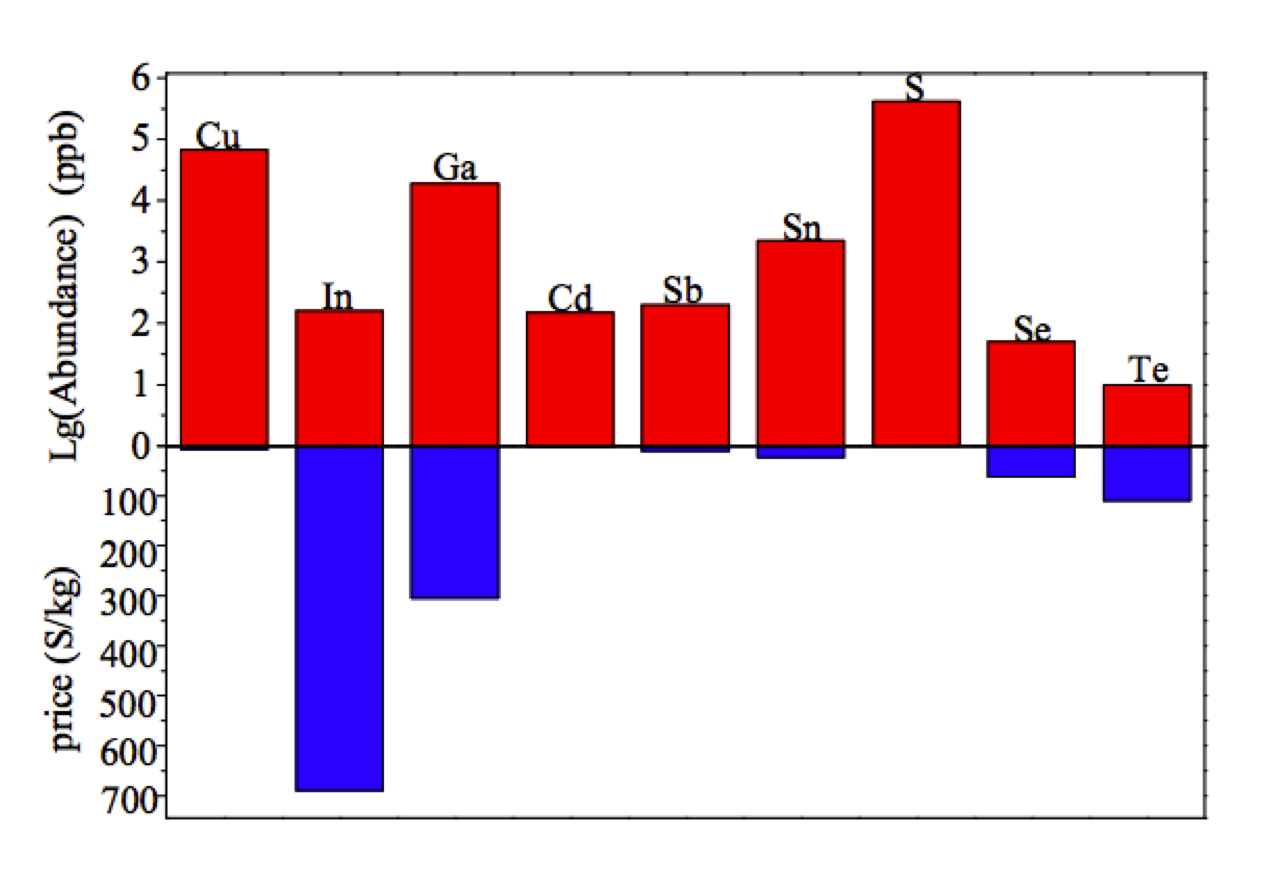
\includegraphics[width=0.7\textwidth]{figures/abundance.png}
    \caption{Comparison of element abundance and price between Cu, In, Ga, Cd, Sb, Sn, S, Se and Te. Figure taken from the supporting information of reference \citenum{Shiyou}, where data was taken from the London Metal Exchange LME.}
  \label{abundance}
\end{figure}

The first candidate photoferroelectric material, enargite (\enargite), is a mineral that corresponds to a semiconductor of type $A^I_3B^VC^{II}_4$, and is frequently found as an impurity in copper ores \cite{enargite_EIS}.
Minerals of the composition $Cu_3(As,Sb)S_4$ are known to occur in two polymorphs: tetragonal with sulfur in cubic close packing or orthorhombic with sulfur in hexagonal close packing. In both cases the coordination is tetrahedral for all atoms \cite{ores}. Enargite is the most common member of this group of minerals, its unit cell (as shown in figure \ref{unit_cells}a) has an orthorhombic crystal structure with space group $Pmn2_1$ and chemical composition \enargite with  a small percentage of Sb \cite{ores1}. The main impurities in natural enargite are Sb and Fe, but Pb and Ag are also known to be present to some extent \cite{enargite_EIS}.
Natural samples of enargite have been found to exhibit the electrical properties of a p-type doped semiconductor with a conductivity of  0.0014 S/m (from the stated value of approximately 7 $\Omega$ cm for the resistivity at 295 K) \cite{enargite_properties}. In the same work, two optical transitions were determined: an indirect one at 1.19 eV and a direct one at 1.44 eV. Although more recent studies have given a value of 1.28 eV for the band gap of enargite from measurements of temperature dependent resistivities, diffuse reflectance spectroscopy and photoacoustic spectroscopy  \cite{Dittrich1}. A theoretical study using the first principles quasi-particle GW method based on wavefunctions generated from the hybrid functional HSE06 \cite{HSE}, has predicted a value of 1.32 eV for the band gap \cite{Zunger}. Although a number of different values have been reported for the band gap of enargite, all values stated fit within the optimal range of 1.06 eV to 1.50 eV \cite{CZTS_book} for a solar absorber material.\\

\begin{figure}[h!]
  \centering
    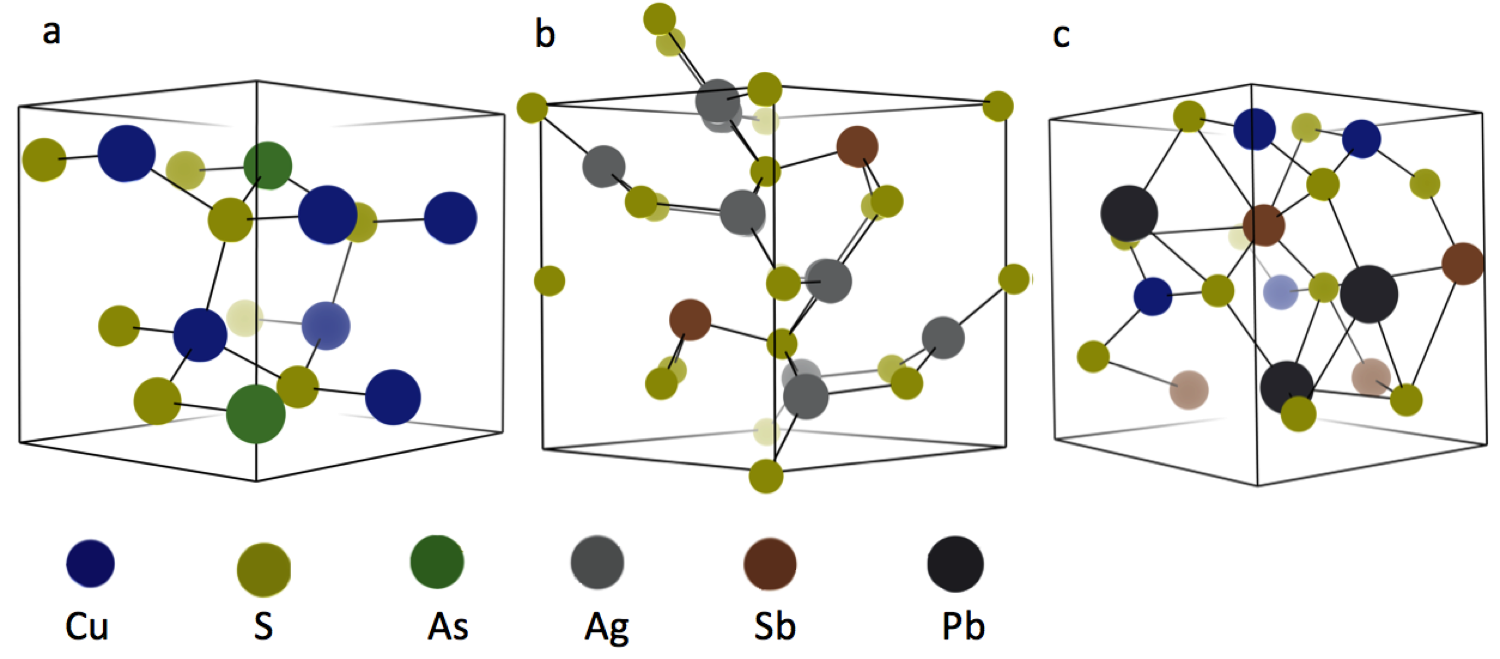
\includegraphics[width=1.0\textwidth]{figures/unit_cells.png}
    \caption{The 15 atom primitive unit cell of enargite (\enargite) (a), 19 atom primitive unit cell of stephanite (\stephanite) (b) and 23 atom primitive unit cell of bournonite (\bournonite) (c).}
  \label{unit_cells}
\end{figure}

The unit cell of the second candidate photoferroelectric material, stephanite (\stephanite), also has an orthorhombic crystal structure but with space group $Cmc2_1$, and is shown in figure \ref{unit_cells}b. 
The structure is composed of columns of $SbS_3$ pyramids extended along the z axis. The columns are located pairwise; in each column, pyramids occupied with antimony atoms alternate with empty pyramids. The Sb-S distances in the pyramids are 2.48, 2.42, and 2.42 $\AA$. Silver atoms are located in the tetrahedral coordination between $SbS_3$ groups (at the centers of rhombic channels). Three types of $AgS_4$ tetrahedra with different Ag-S distances can be identified. The distinctive feature of the structure is a large number of common edges of Ag tetrahedra \cite{stephanite}.
It has been reported that stephanite has a band gap of 1.62 eV \cite{Dittrich1}. Otherwise, there is seemingly very little information available in the literature on the optical or electrical properties of stephanite apart from a work in 1973, given in reference \citenum{stephanite_old}, showing the electrical resistivity of a synthetic sample of stephanite as a function of temperature. The work measures a resistivity of approximately 9 $\Omega$ cm for the stephanite sample at 110 $^\circ$C, which corresponds to a conductivity of 0.0011 S/m. There has also been some speculation in the literature on the possibility of ferroelectric behaviour in stephanite due to the presence of ferroelectric phases at very low temperatures in pyrargyrite ($Ag_3SbS_3$), proustite ($Ag_3AsS_3$) and stibnite ($Sb_2S_3$), which are crystallochemically related to stephanite \cite{stephanite}. The same study also notes that similar displacement structural changes occur in stephanite to those in proustite and pyrargyrite that are responsible for the ferroelectric properties of these materials.\\

Similarly, up until very recently, little information has been available on the optical or electrical properties of the third candidate photoferroelectric material, bournonite (\bournonite). Bournonite also has an orthorhombic crystal structure and the same space group as enargite,  $Pmn2_1$, with measured values of 1.23 eV \cite{Dittrich1} and 1.31 eV \cite{bournonite} reported for the band gap. However, very recently this material has received increasing scientific interest for thermoelectric and rewriteable data storage applications due to a measured low thermal conductivity \cite{Dong}. 
Consequently, works on the synthesis of bournonite are beginning to emerge such as that in reference \citenum{bournonite}.
The low thermal conductivity of bournonite has been attributed to the distortive environment of the Pb and Sb atoms from the stereochemically active lone-pair $s^2$ electrons \cite{Dong}. In the same study they perform electronic structure calculations to predict the band structure of the material, however in the study they use only the generalized-gradient approximation (GGA) level of accuracy in density functional theory for their calculations, which is know to underestimate the band gap of a semiconducting material. They do however show that the inclusion of spin-orbit coupling (SOC) has a considerable impact on the calculated band gap of the material. In the study they predict a direct band gap of 0.686 eV before including SOC and two optical transitions when they do include SOC: a direct band gap of 0.445 eV and an indirect band gap of 0.385 eV. Different levels of accuracy in DFT electronic structure calculations and the impact of SOC on the optoelectronic properties of a material are discussed further in sections \ref{DFT_section} and \ref{SOC_section} respectively. 
A more reason study has made use of DFT+U methodology to avoid the underestimation of the band gap when calculating the optoelectronic properties of this material, where they predicted a band gap of 1.22 eV \cite{bournonite_new}. There was however no mention of SOC in the study, which was shown in the older study to influence to band structure of the material considerably, and the limitations of DFT+U methodology are discussed in section \ref{DFT_section}.\\


\begin{table}[]
\centering
\caption{Summary of known key properties of the three candidate photoferroelectric materials from the literature.}
\label{properties}
\begin{threeparttable}
\begin{tabular}{lllll}
\toprule[1.2pt]
\multicolumn{1}{l}{Candidate} & \multicolumn{1}{l}{Empirical Formula} &  \multicolumn{1}{l}{Space Group} & \multicolumn{1}{l}{Band Gap (eV)} & \multicolumn{1}{l}{Conductivity (S/m)} \\ \midrule[1pt]
Enargite                      &     \enargite         &                                $Pmn2_1$  & 1.28 \cite{Dittrich1}                 & 0.0014 \cite{enargite_properties} \tnote{ii}                           \\
Stephanite                    &   \stephanite &                                $Cmc2_1$ & 1.62  \cite{Dittrich1}                    & 0.0011 \cite{stephanite_old} \tnote{ii}                                    \\
Bournonite                    &      \bournonite  &         $Pmn2_1$                &          1.23 \cite{Dittrich1}, 1.31 \cite{bournonite}                        & -                                     
 \\ \bottomrule[1.2pt]
\end{tabular}
\begin{tablenotes}
\item[i] From resistivity of a natural sample measured at 295 K \item[ii] From resistivity of a synthetic sample measured at 383 K
\end{tablenotes}
\end{threeparttable}
\end{table}

The key known experimentally derived properties of the three candidate materials that were described above are summarised in table \ref{properties}. In this study we aim to use the highest level of theory possible to calculate as many of the properties relevant for a solar absorber material as possible, which were discussed in section \ref{PV_properties}, in order to determine if these materials are likely to perform well in this application. Firstly we use hybrid-DFT electronic structure calculations to optimize the crystal structure of a bulk system, starting from the highest quality X-Ray diffraction data available for the materials. From this we calculate the band structures of the materials to determine the size of the band gap and whether it is direct or indirect in nature as this would be a good indicator of how strongly the materials will absorb sunlight. We then go on to calculate the dielectric function and optical absorption coefficients of the materials...


